\documentclass[12pt,a4paper]{report}
\usepackage{amsmath}
\usepackage[hidelinks]{hyperref}
\usepackage{comment}
\usepackage{graphicx}
\usepackage{placeins}

\usepackage[left=2.50cm, right=2.50cm, top=2.50cm, bottom=2.50cm]{geometry}
\graphicspath{{./Images/}}

\begin{document}
	
	\author{Compliance Design of Automotive Systems \\
		a.y. 2020/2021\\\\
		Group Members:\\
		Barro Alessandro, Bruscoli Nicolas, Ceccarelli Viviana, \\
		Chiacchiararelli Leonardo, Cintura Manuel, Mariani Lucia\\
	}
	\title{Project Report\\
		Adaptive Cruise Control
	}
	\maketitle
	
\tableofcontents
\listoffigures


\chapter{Introduction}
The reason for the choise of the Adaptive Cruise Control is because is one of the most used feature of the ADAS. ADAS (Advance Driver Assistance Systems) are the electronic systems that assist drivers in driving and parking functions. ADAS increases car and road safety, uses automated technology, such as sensors and cameras.\\ More and more vehicles are equipped with it, often as standard, and the Adaptive cruise control is one of the most advanced technology and able to facilitate the driving.\\
Adaptive cruise control (ACC) is an active safety system that automatically controls the acceleration and braking of a vehicle. It is activated through a button on the steering wheel and cancelled by driver’s braking and/or another button.
The report offers an example that illustrates the benefits of using the Model-Based Design in the engineering workflow.
The goal is to show how this approach can be used in the entire development of the system design.\\
The report is divided in these following section:
\begin{itemize}
	\item in $Chapter 2$ there is Project organization, where it is explains the model based design and the team organization
	\item in $Chapter 3$ it is offers the Model explanation and design of the Adaptive cruise control
	\item in $Chapter 4$ there are all the various steps for the project development. Starting from the Unity test, then with the MIL, the automated generated code and then with the SIL and PIL simultion.
	\item Finally, in $Chapter 5$ there is the conclusion with the future developments.
\end{itemize}

\chapter{Project organization}
\section{Hardware and software components}
All the hardware and software components used to realize the prrject are listed here:
\subsection{Hardware}
The hardware used for this project is rather simple: PC running Windows and a Raspberry Pi 4 Model B.\\
The Raspberry has been used as core component of the processor in-the-loop simulation.
\subsection{Software}
Software employed for this project is Simulink: Embedded Coder package, Simscape package, Powertrain Blockset are required.
Software employed to organize the work and the communication between team members:
\begin{itemize}
	\item GitHub
	\item LaTeX: for the realization of the documentations
	\item Microsoft Teams: for the meetings
	\item Draw-io: for the graphs realization
\end{itemize}
\section{Model based design}
The realization of the project is based on the V-model, which is one of the most used approaches in the model-based design. The V-Model demonstartes the relationships between each phase of the development lif cycle and its associated phase od testing.  The horizontal and vertical axes represents time or project completeness (left-to-right) and level of abstraction, respectively. \\
\begin{figure}[htbp]
	\centering
	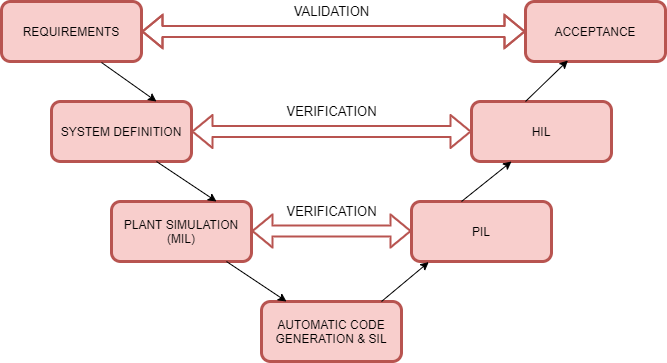
\includegraphics[scale=0.6]{v-model.png}
	\caption{The V-model}
\end{figure}
\FloatBarrier
The project definition phases are:
\begin{itemize}
	\item \textbf{Requirement}: evaluation of the model requirements, planned how to proceed with the following steps and fixed the final goals.
	\item \textbf{System definition}: define the high-level design for the model.
	\item \textbf{Plant simulation}: it is realized the simulation of the plant using Simulink.
	\item \textbf{Automatic code generation}: using Embedded Coder to generale the low-level code for the controller.
	\item \textbf{PIL}: the code generated was deployed to hardware, and the processo in-the-loop has been performed.
	\item \textbf{HIL}: here, the plant should be simulated in HIL module. This step, due to the available instrumentaions, it could not be implemented.
	\item \textbf{Acceptance}: the real plant is realized, integration tests are performed. Again, no possibility to perform this step.
\end{itemize}
\FloatBarrier
\section{Team organization}


\chapter{Model explanation \& design}
As anticipated before, the aim of this project is to design an Adaptive Cruise Control: to design it following the MBD, we of course need a plant that models the vehicle longitudinal dynamics.
In Fig \ref{Plant} it is possible to see the whole plant model.

\begin{figure}[htbp]
	\centering
	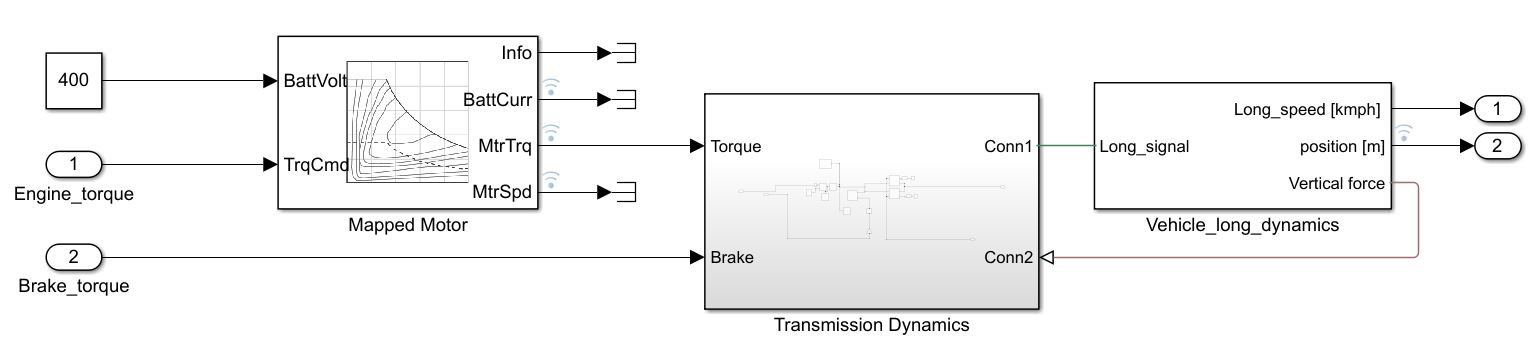
\includegraphics[scale=0.5]{Plant.jpg}
	\caption{Plant}
	\label{Plant}
\end{figure}


Going deeper, it is possible to see that it consists of three main blocks:

\begin{itemize}
	
	\item Vehicle longitudinal dynamics block;
	
	\item Transmission dynamics block;
	
	\item Mapped motor block.
	
\end{itemize}

Let us start the description from this last block.

\section{Mapped motor}

This first block is used to implement a mapped motor and drive electronics operating in torque control mode: the output torque tracks a reference demand one, directly coming from the output of the PID controller. This torque will be one of the possible input of the next block, the Transmission Dynamics one. Particularly, from the output of the PID controller we could have a positive torque if the vehicle needs to accelerate, or a negative torque if the car needs to brake: the first one will be above mentioned input of the Mapped Motor block, the latter one will be directly applied to the brake system in the Transmission Dynamics block.

\section{Transmission Dynamics}



Thanks to this block it is possible to model the entire driveline, from the ECU torque request to the wheels motion.
 
 \begin{figure}[htbp]
 	\centering
 	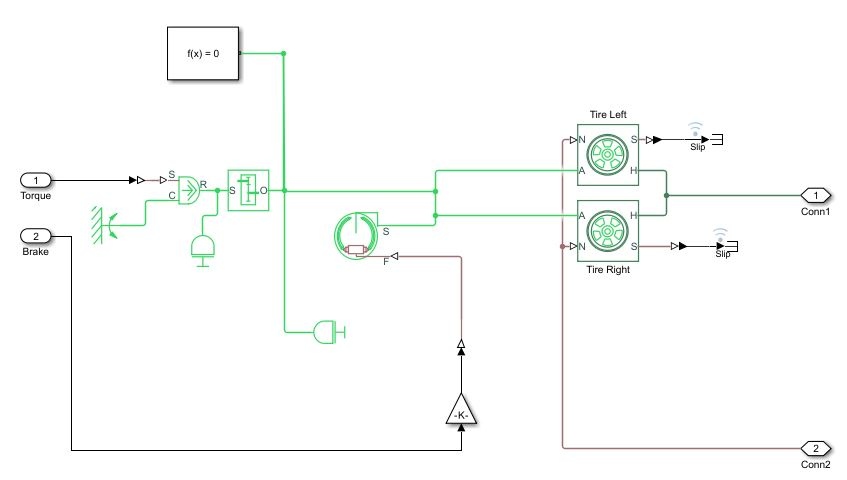
\includegraphics[scale=0.8]{TransmissionDynamics.jpg}
 	\caption{Transmission Dynamics block}
 \end{figure}

As anticipated before, this block has two inputs:
\begin{itemize}
	
	\item The positive torque input, output of the Mapped motor block; 
	
	\item The negative torque input, output of the PID controller.
	
\end{itemize}

In the first case, the torque is modified by a gear ratio block which models the one-speed transmission of the electric vehicle. Conversely, when a negative torque is asked, the brake block provides a negative torque directly at the wheel input. Then, the Simscape wheels blocks model the behaviour of the wheels in terms of inertia, rolling resistance and slip, giving us an angular speed of the wheel that is proportional to the torque given as input.

\section{Vehicle longitudinal dynamics}


Finally, to model the longitudinal dynamics of the vehicle, from the Simscape Driveline library the “vehicle longitudinal dynamics” block was picked.


\begin{figure}[htbp]
	\centering
	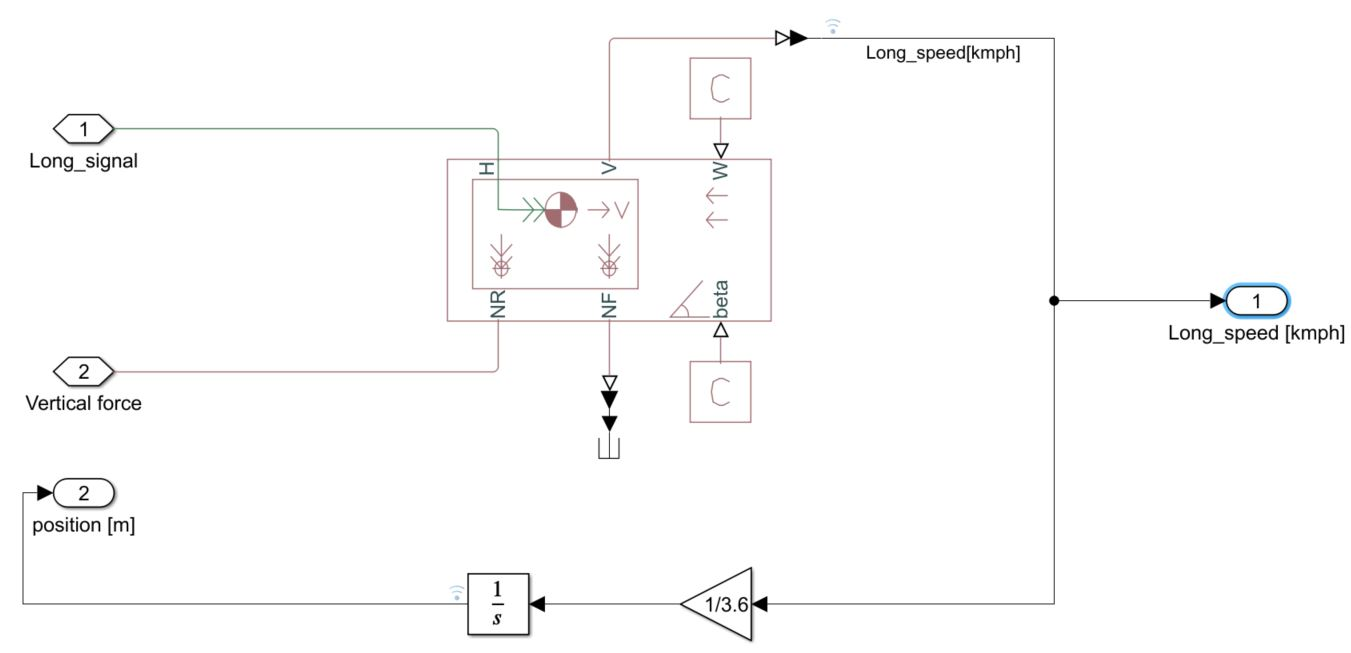
\includegraphics[scale=0.5]{LongitudinalDynamic.jpg}
	\caption{Vehicle longitudinal dynamics block}
\end{figure}

This block represents a two-axle vehicle body in longitudinal motion: it accounts for body mass, aerodynamic drag, road incline, headwind speed (in our simulations they are not considered influencing quantities)and weight distribution between axles due to acceleration and road profile. The block accepts as input the resulting traction motion developed by tires (that is to say, the output of the Simscape wheels blocks), giving as output the vehicle velocity and also the front normal wheel forces.\\
Finally, from this block is also emulated the radar function, that is to say the monitoring of the distance between this vehicle and the first one: in fact, thanks to the presence of an integrator block, from the actual speed of the vehicle its position is computed. Then this position is fed back and subtracted to the position of the first vehicle, giving us the resulting radar distance.

\begin{figure}[htbp]
	\centering
	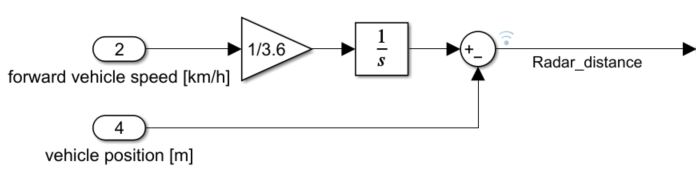
\includegraphics{RadarFunction.jpg}
	\caption{Emulation of the radar function}
\end{figure}



\chapter{Project development}

\section{Requirements}
\subsection{Software requirements}

In order to be able to interact with the developed model, some software tools are needed:

\begin{itemize}
	
	\item Matlab R2019b;
	
	\item Simulink;
	
	\item Simscape;
	
	\item Simscape Driveline.
	
\end{itemize}

\subsection{High level requirements}

The goal of the overall control system is to extend the mission of the simpler Cruise Control: regulate the speed to the desired one and keep it. In addition respect this goal, the Adaptive Cruise Control adapts the speed of the vehicle respect the velocity of the following one, being able to correctly mantain the safety distance dictated by the Highway Code when it needed (that is to say, when the current distance between the vehicles is lower than the required safety distance):

\begin{equation*}
	d_s=d_{min}+\dfrac{1}{k}v^2
\end{equation*}

\begin{figure}[htbp]
	\centering
	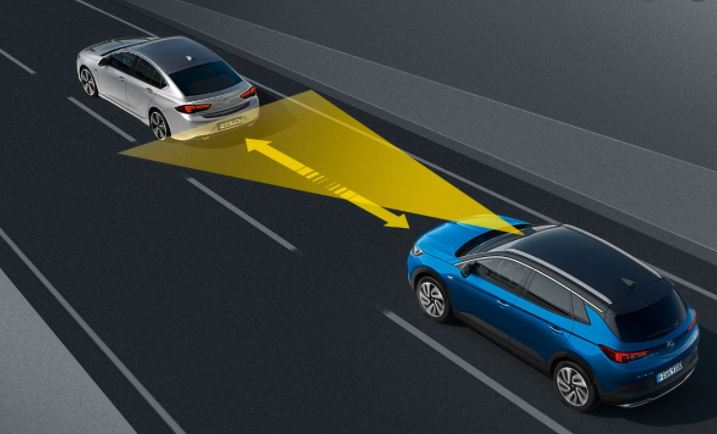
\includegraphics{ACC.jpg}
	\caption{ACC}
\end{figure}

\subsection{Low level requirements}
The designed system is intended to work on an electric vehicle, considering also the state of charge of the battery: particularly, the overall behaviour of the control action will be more or less aggressive depending on the state of charge level.

\begin{figure}[htbp]
	\centering
	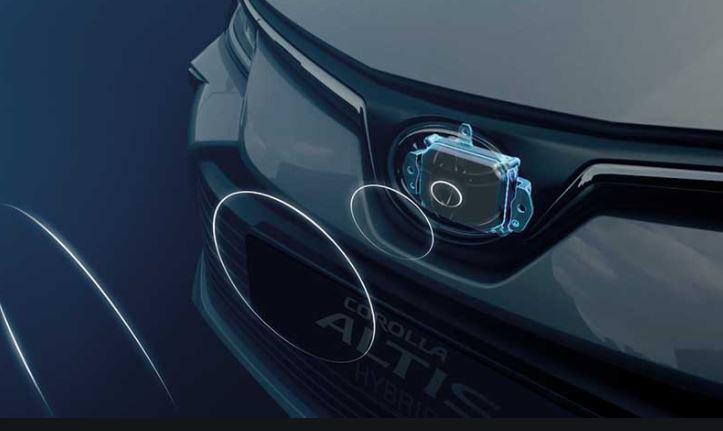
\includegraphics{RadarACC.jpg}
	\caption{Front radar}
\end{figure}

Thanks to the presence of a sensor (typically a radar installed in the front of the car), the distance respect the following vehicle is continuosly monitored: when this distance falls below the threshold dictated by the Highway Code minus a safety margin quantity (one meter as dictated by requirement, to be sure to be able to brake in the correct timings), the control must act on the brakes. Then, during the acceleration phase, the system needs to be designed as following: when the first vehicle accelerates, the control must operate so that the vehicle speed becomes the one desired if it is possible,  that is to say if the two vehicles are far enough. Otherwise, the system must adequate the vehicle speed to the one needed to keep the safety distance.




\section{Unity \& Integration testing}
\begin{figure}[!h]
	\centering
	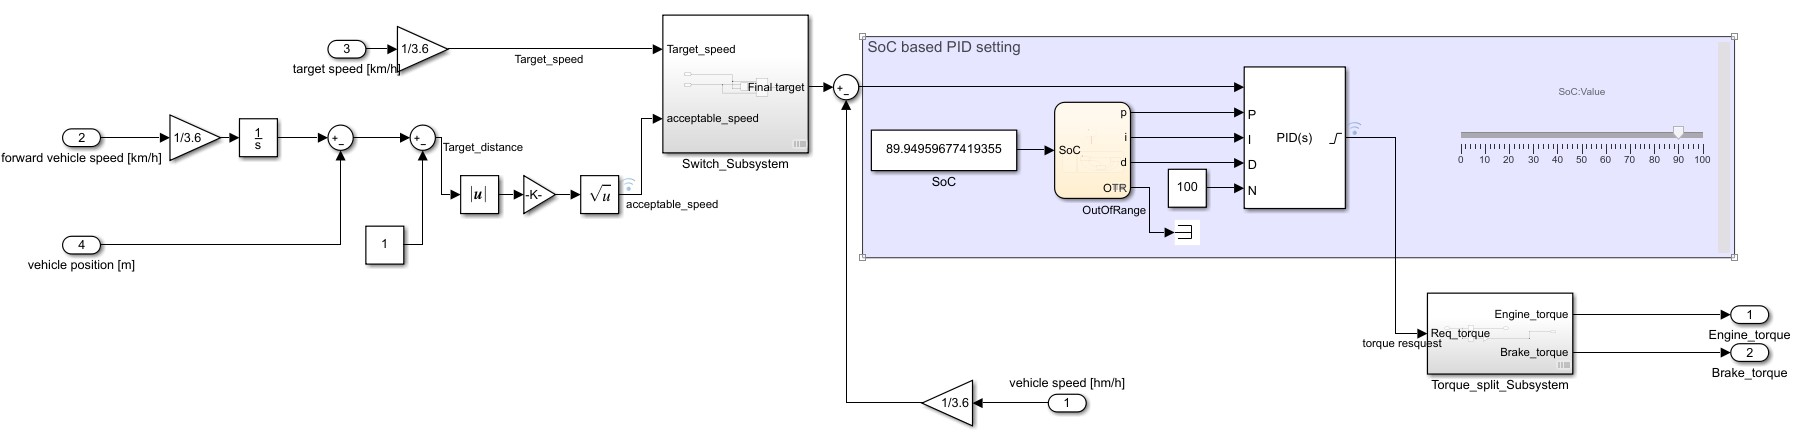
\includegraphics[scale=0.34]{Controller_overview.jpg}
	\caption{An overview of the controller block}
	\label{Controller_overview}
\end{figure}
Our controller is composed by 4 main blocks: switch\_subsys, SoC handler, torque\_split and the PID regulator.
While it is impossible to test the PID behaviour without a model to be controlled, it is necessary to test separately the other blocks.
We tested the units using the tool Simulink Test. We first built an harness for each unity to isolate it from the rest of the model, then we built the input signals in such a way to stimulate the unity in all possible conditions. We also built the baseline signals to tell the tester what output we expected when feeding the unity a given input. 
\newpage
\subsection{Switch subsystem}
\begin{figure}[!h]
	\centering
	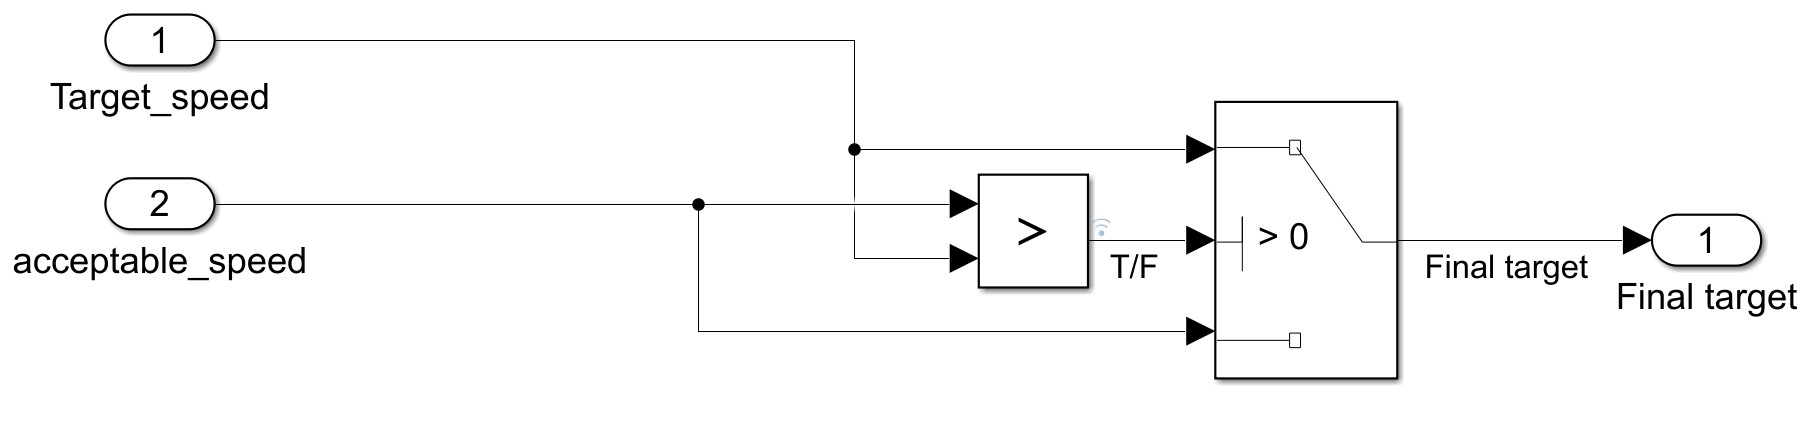
\includegraphics[scale=0.34]{switch_subs.jpg}
	\caption{An overview of the switch subsystem}
	\label{switch_subs}
\end{figure}
\FloatBarrier
This system is composed of a switch commanded by a majority operator fed with the same signals that have to be switched. We wanted to be shure that this small unity would behave as expected. 
In Fig \ref{IO_baseline_switch_detach} we can see the inputs that we used to test the unit: we wanted to test all the possible conditions for the ‘grater than’ block. To better visualize which signal was let go by the switch we tried to differentiate as much as possible the two inputs.
\begin{figure}[!h]
	\centering
	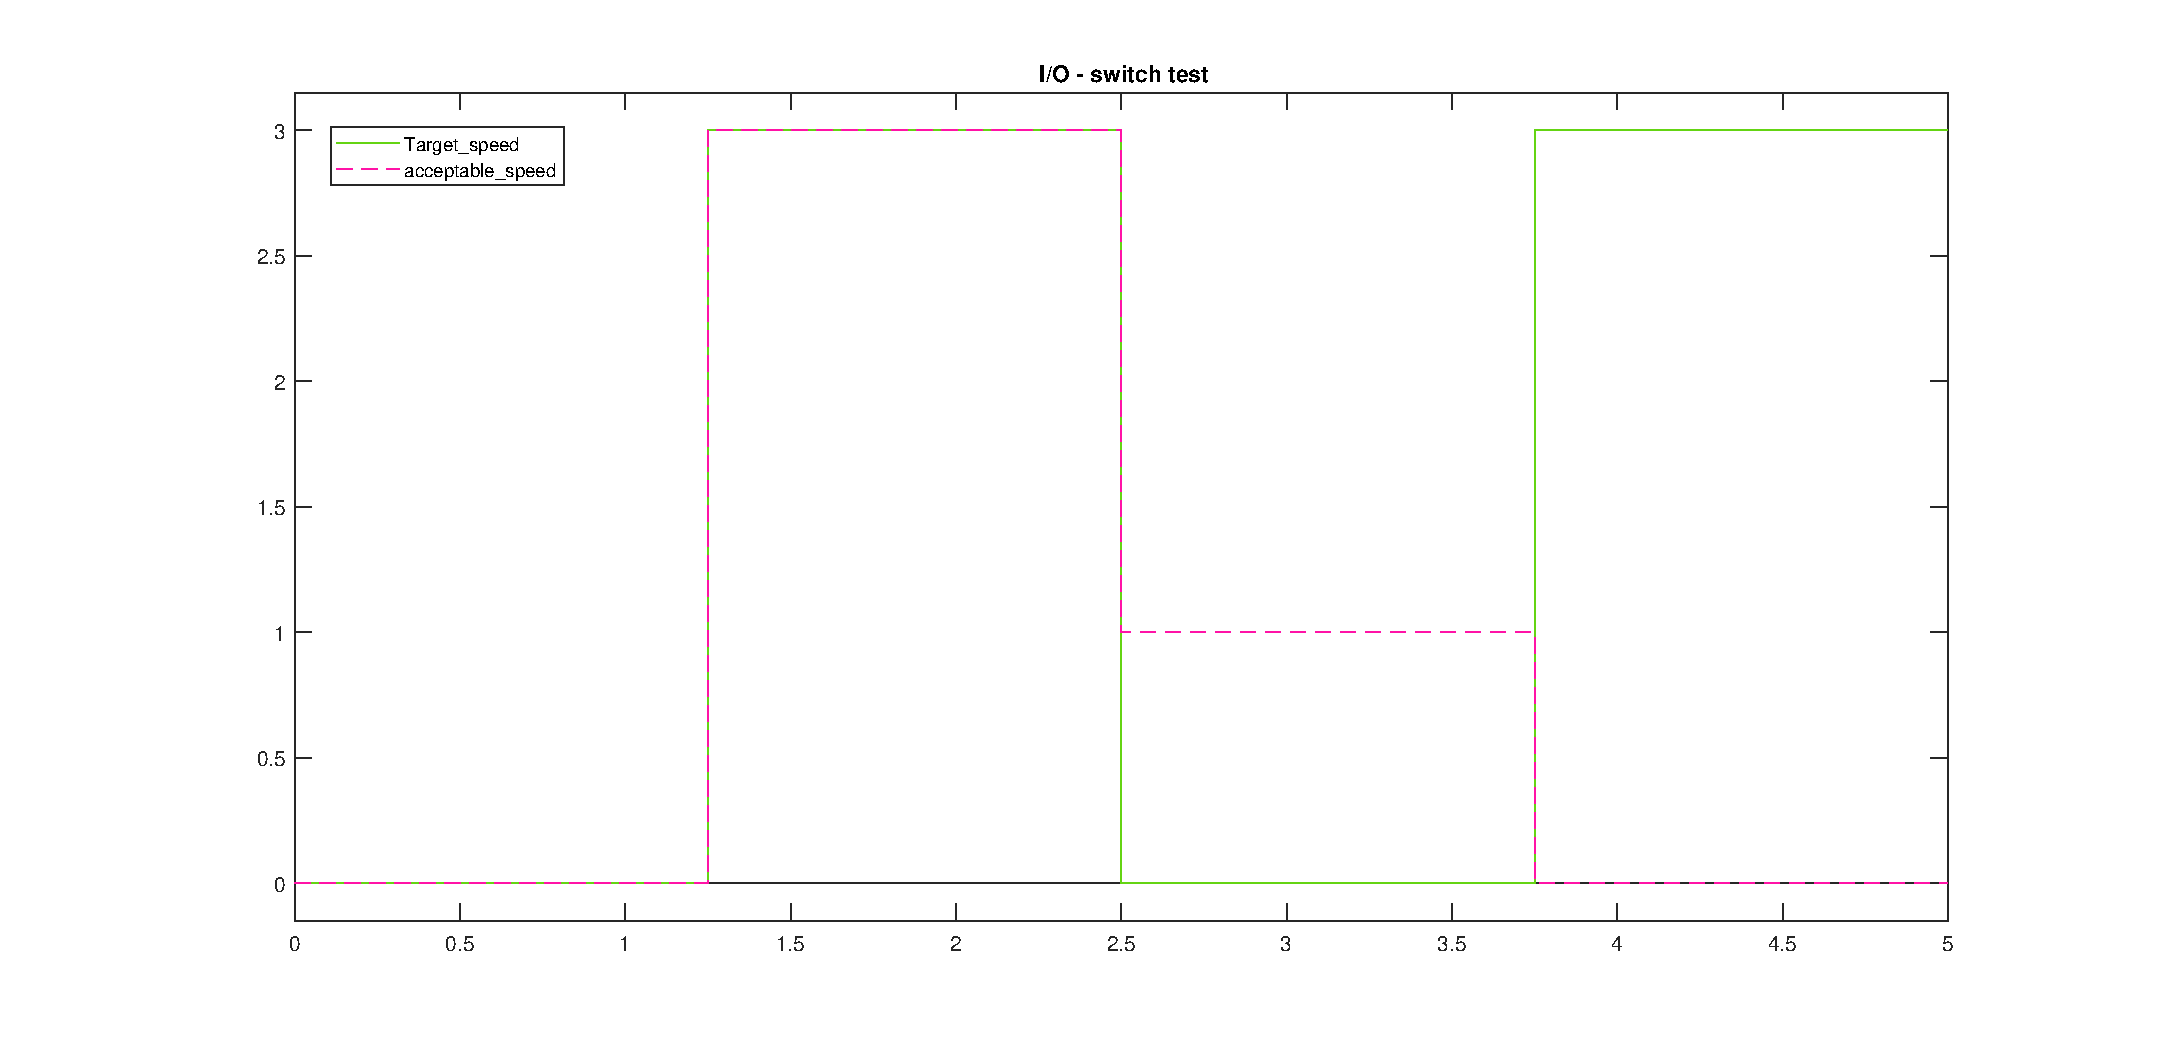
\includegraphics[scale=0.4]{IO_baseline_switch_detach.eps}
	\caption{Inputs of the test: acceptable speed is the one set by the user, target speed is the one of the care ahead}
	\label{IO_baseline_switch_detach}
\end{figure}
As we can see Fig. \ref{switch_baseline} (right) the Simulink test tool is able to generate a document reporting the configuration of the test, to guarantee to the customer (we can call costumer whoever will need to use our subsystem and will need it being tested) that the test was performed accordingly to his needs. This feature also gives the opportunity to an external part to perform the exact same test and verify that the results are coherent.
In the same way the tool can generate a report regarding the output of the test, here in Fig. \ref{switch_baseline} (left) we can see that the test produces successful results, in fact the output of the test coincides precisely with our baseline signal. 
 %PUT BOTH THE FIGURES IN ONE FIGURE SIDE BY SIDE
\begin{figure}[!h]
	\centering
	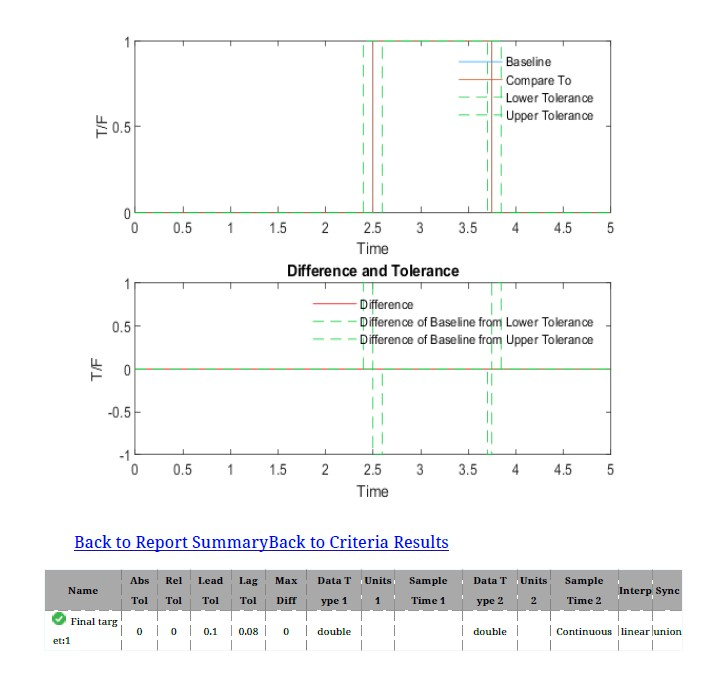
\includegraphics[scale=0.4]{switch_baseline.jpg}
	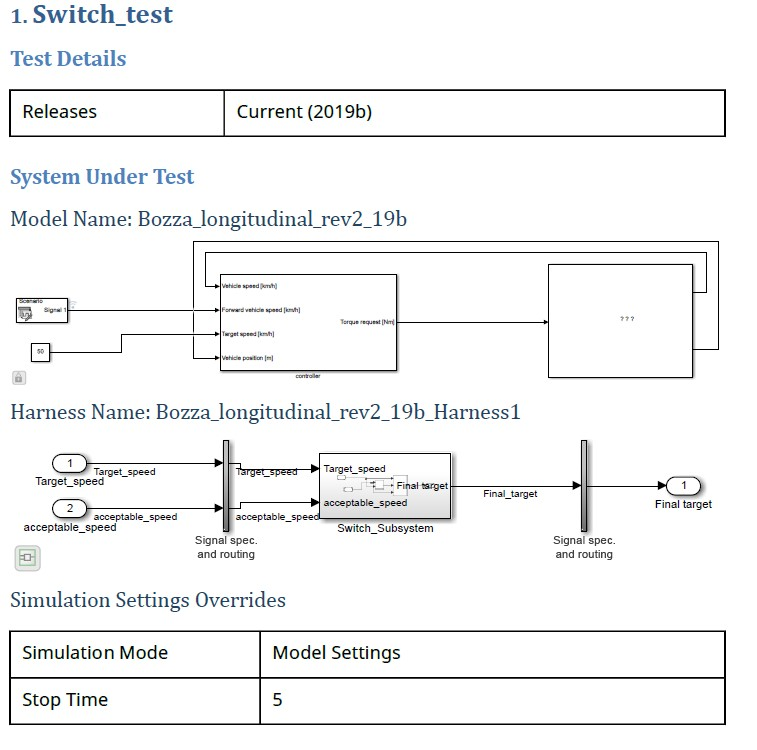
\includegraphics[scale=0.4]{switch_tes_spec.jpg}
	\caption{Automatically generated test reports}
	\label{switch_baseline}
\end{figure}
\FloatBarrier
\subsection{Torque split}
\begin{figure}[!h]
	\centering
	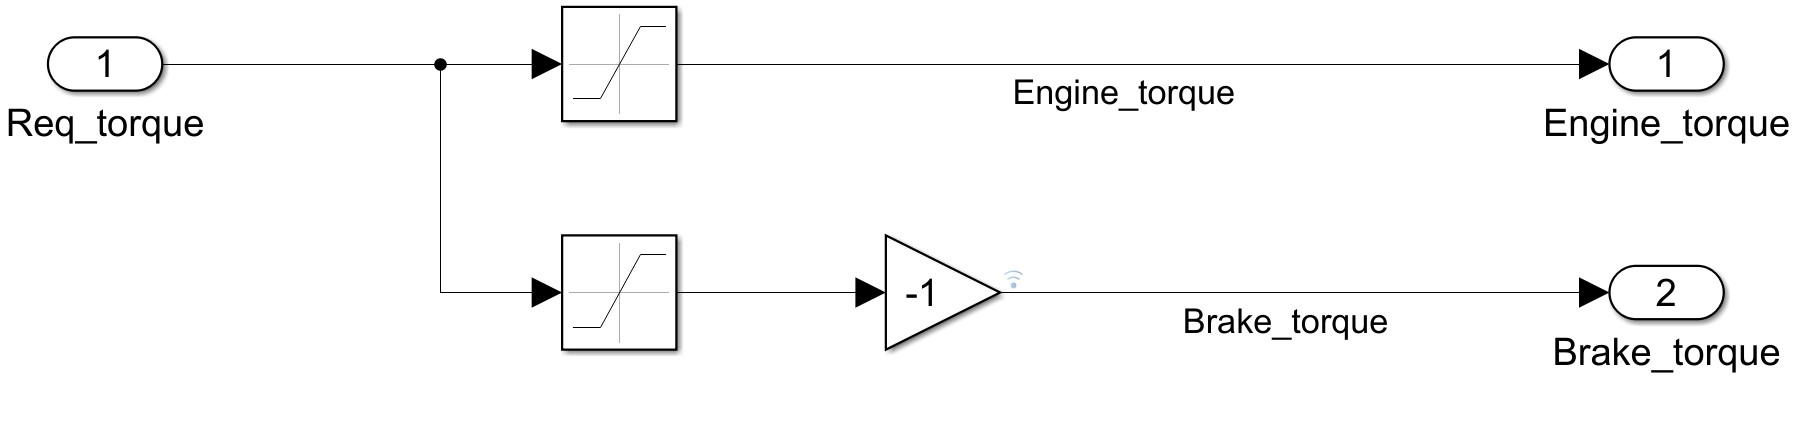
\includegraphics[scale=0.34]{split_subs.jpg}
	\caption{An overview of the torque split subsystem}
	\label{split_subs}
\end{figure}
This unit’s goal is to split the signal coming from the PID, asking for torque. The PID asks for a negative or positive torque, we have to be able to translate the negative torque in a signal to be sent to the brake module. This unit’s goal is to divide the torque signal into two signals depending on the sign of the PID output. To test this unit we just had to verify that when given a positive input it was transferred to output assigned to the engine and when given a negative input it was transferred to the brake output. At the same time the output assigned to the opposite sign has to be zero.
In Fig. \ref{input_split_test} you can see how the test input was designed and you can see that the output corresponds exactly to the baseline signal, meaning a successful test.
\begin{figure}[!hbt]
	\centering
	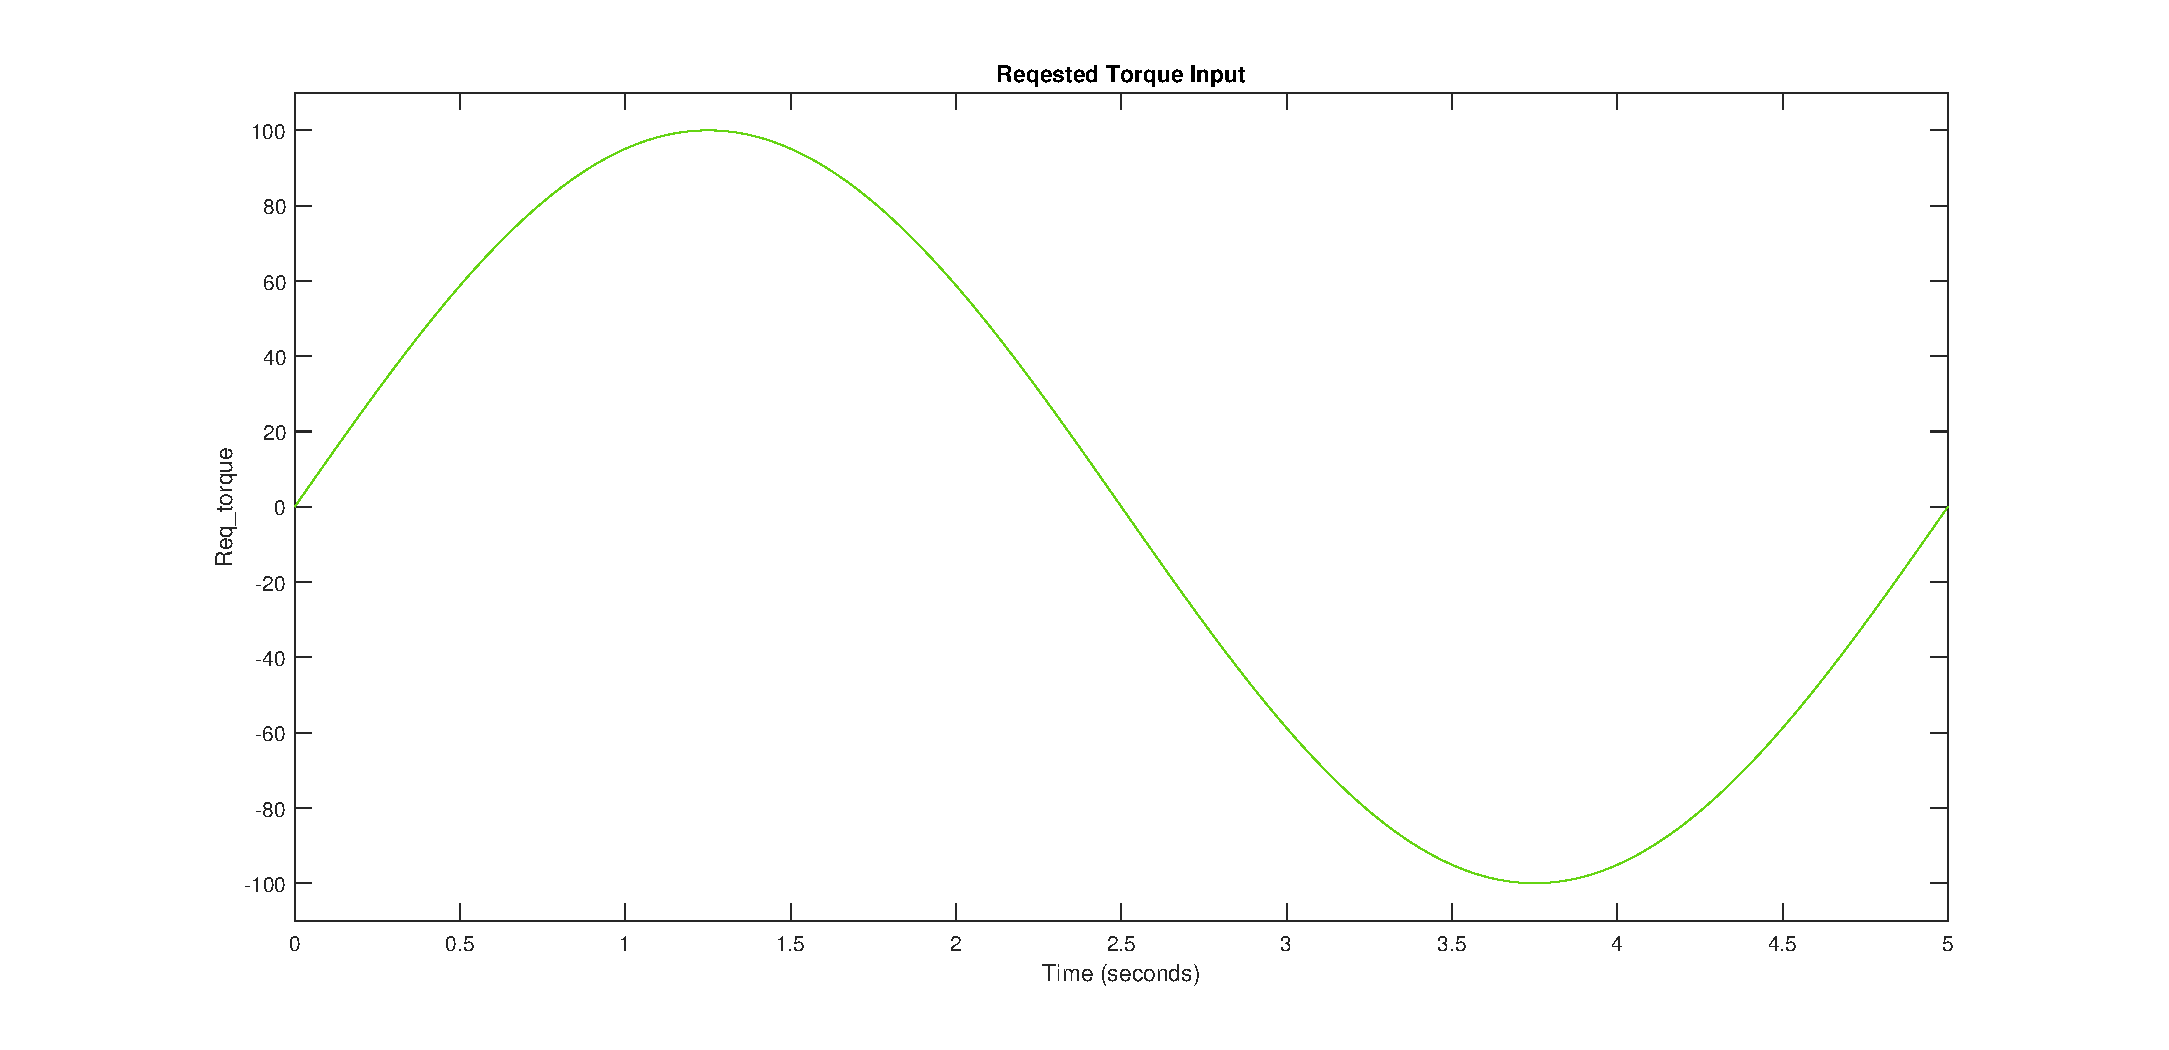
\includegraphics[scale=0.4]{input_split_test}\hfill
	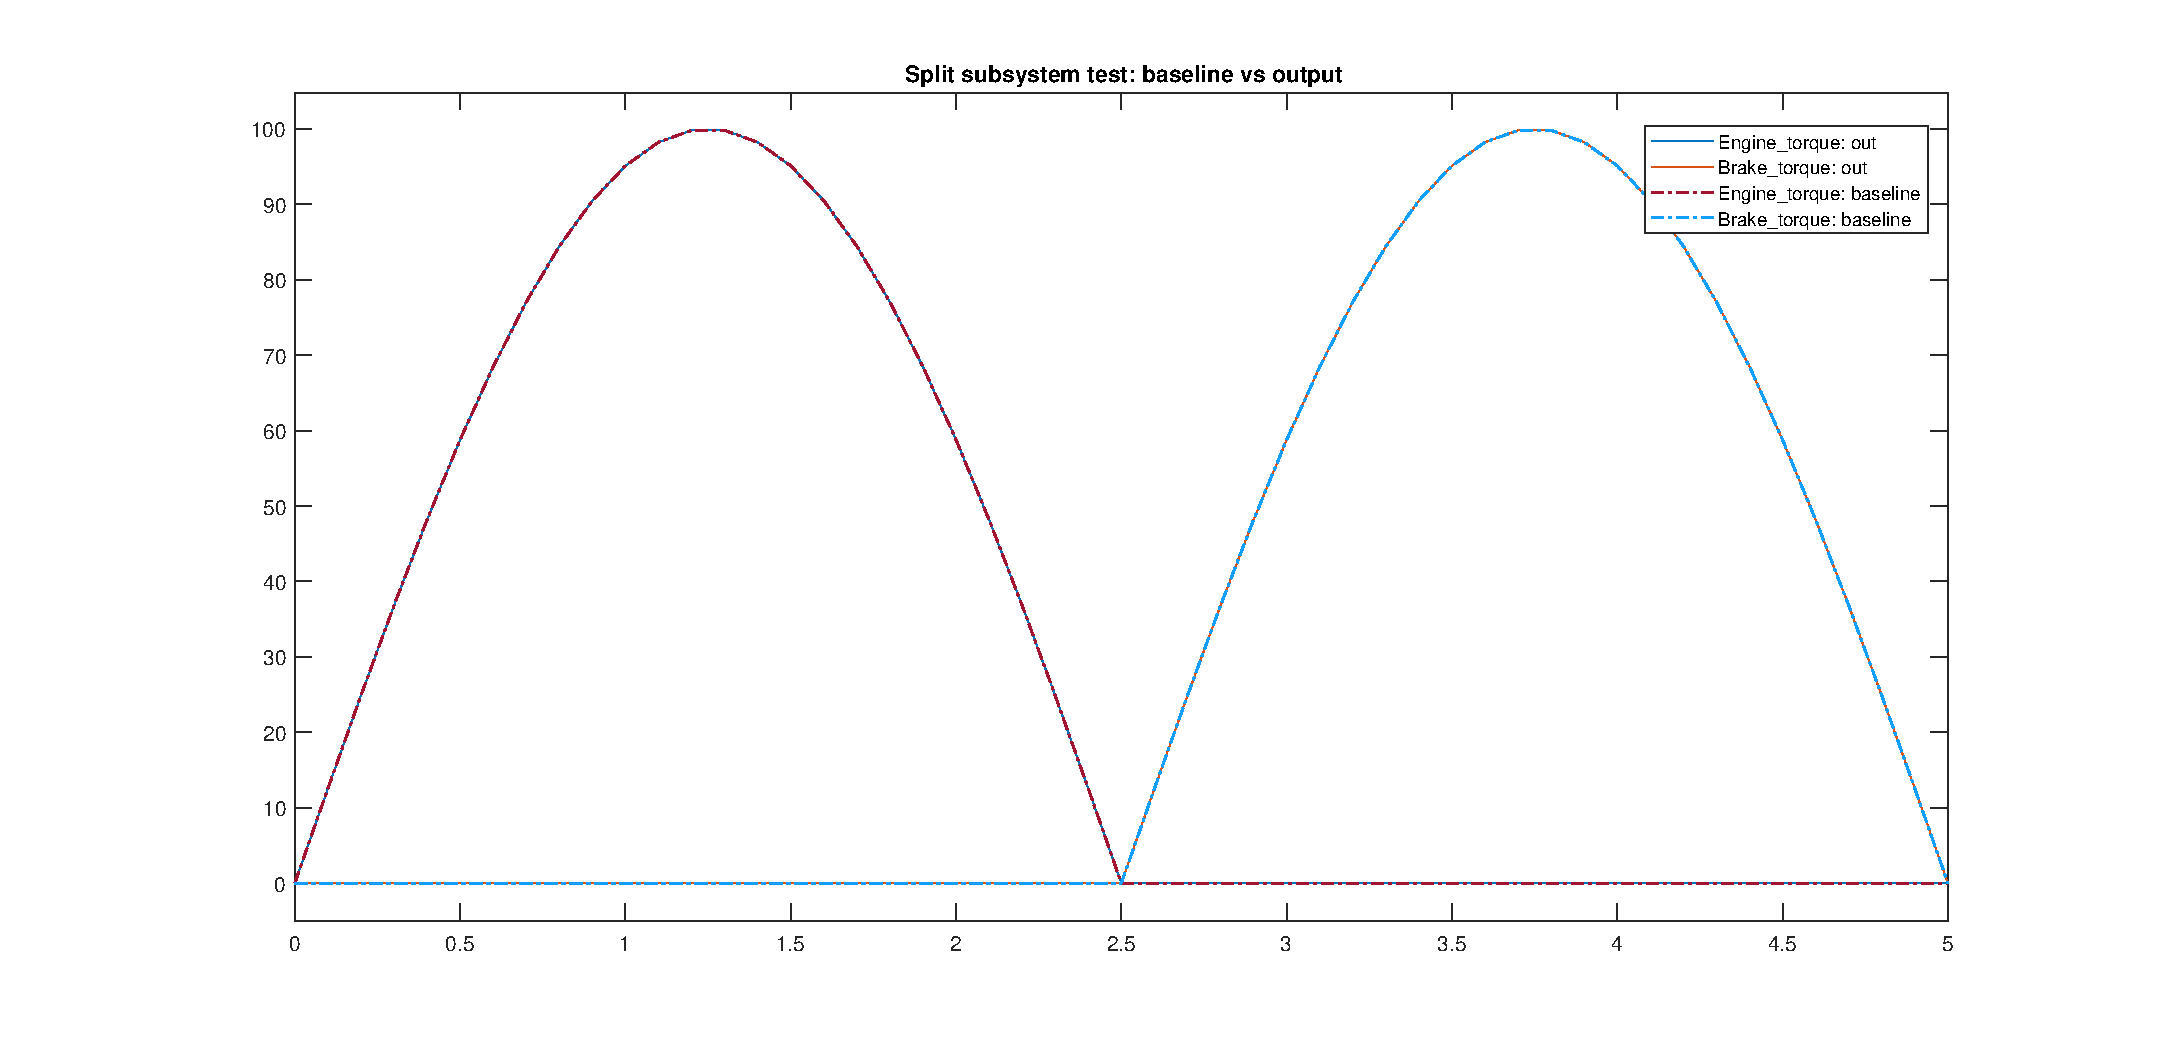
\includegraphics[scale=0.4]{out_split_test}
	\caption{Test inputs (up) Outputs vs baseline (down)}
	\label{input_split_test}
\end{figure}
\FloatBarrier
\subsection{SoC handler}
\begin{figure}[!h]
	\centering
	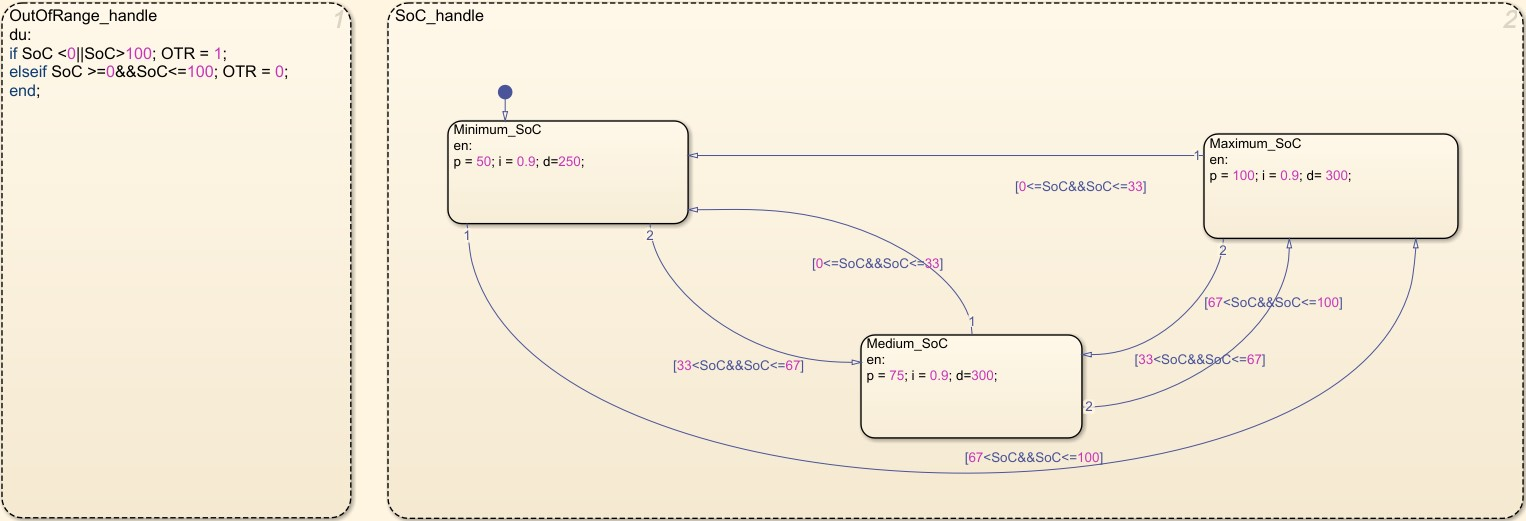
\includegraphics[scale=0.34]{SoC_handle_subs.jpg}
	\caption{An overview of the SoC handler chart}
	\label{SoC_handle_subs}
\end{figure}
\FloatBarrier
This unit is a FSM, so a slightly more complicated test is due. The goal of this unit is to manage the aggressiveness of the control depending on the SoC of the vehicle’s battery pack. We want a less aggressive control if the car has less autonomy left. We divided the interval of possible SoC values in three segments: minimum, medium, maximum. Each segment corresponds to a different state. We have three states, since from each state you can go to the other two we have in total 6 transitions.  We have only one input: SoC signal. In the input signal, wich you can see in Fig.\ref{SoC_handle_input}, we changed the signal in order to stimulate all the possible transitions. 
To be more robust against unexpected behaviour we wanted an additional output for the FSM. The SoC signal is expected to never trespass the 0\% and 100\% bounds, so we created a signal “OutOfRange” that rises when this condition is verified. The FSM is designed to check constantly the OTR signal while performing the ordinary tasks, so a parallel state is created in the FSM.
\begin{figure}[!h]
	\centering
	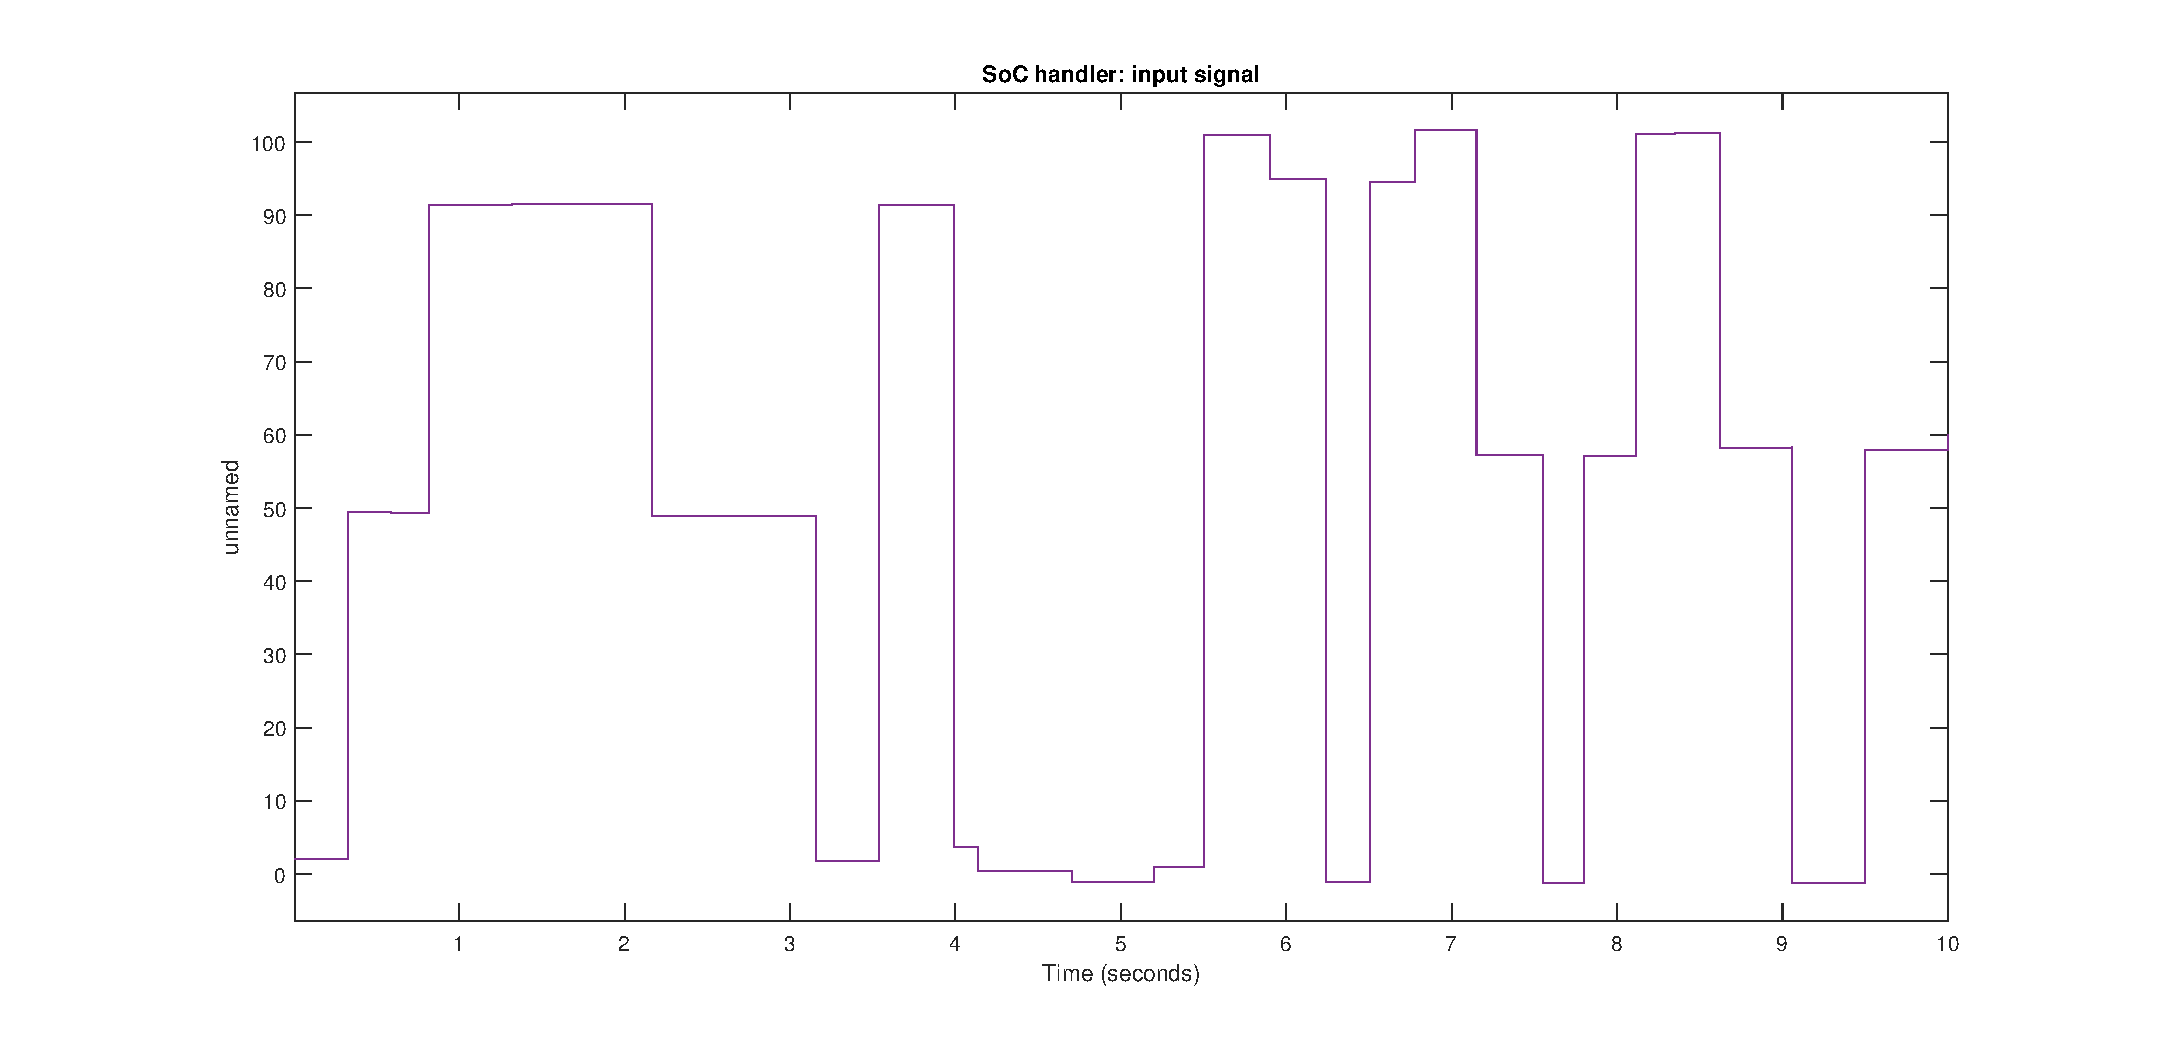
\includegraphics[scale=0.34]{SoC_handle_input.eps}
	\caption{Input fed to the SoC handler }
	\label{SoC_handle_input}
\end{figure}
\begin{figure}[!hbt]
	\centering
	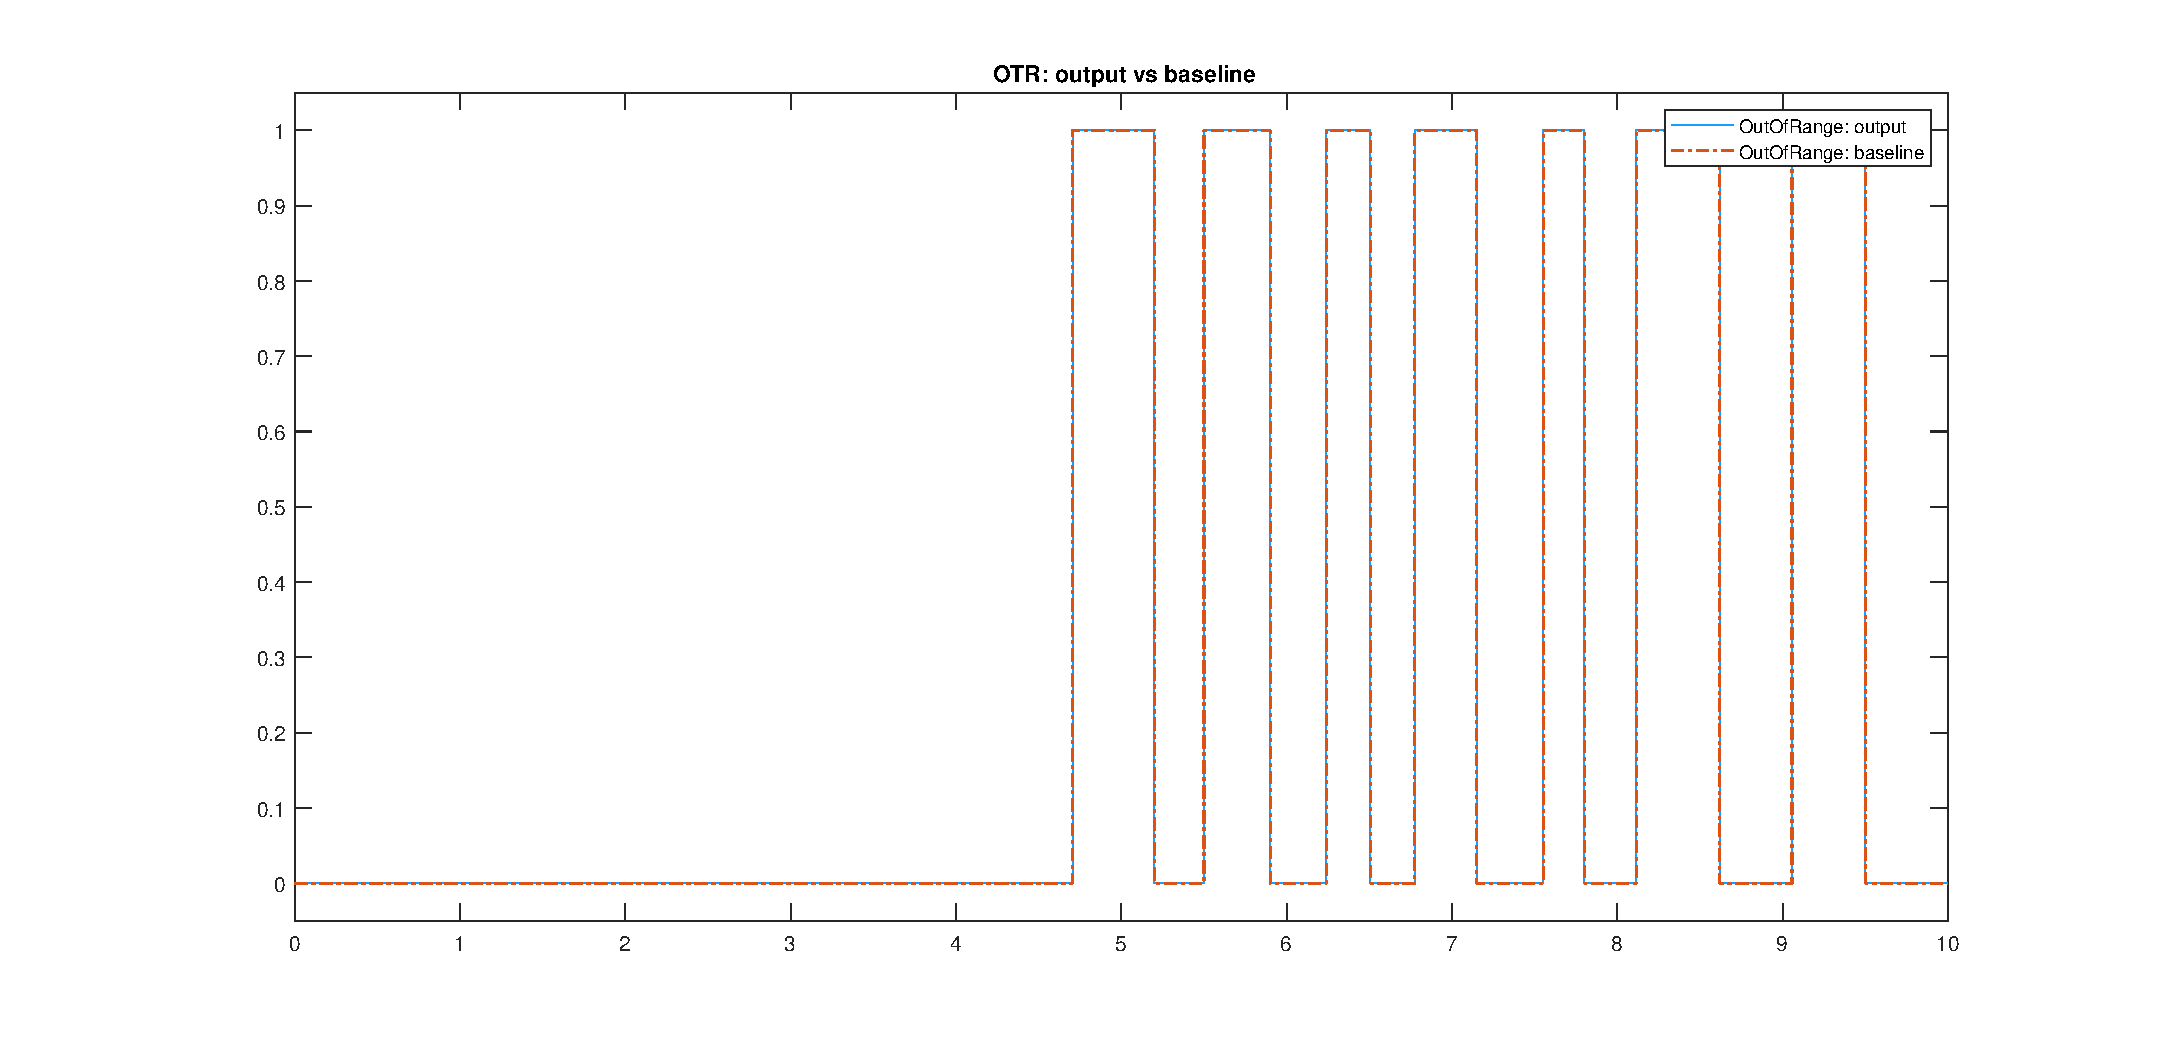
\includegraphics[scale=0.4]{OTR_baseline_result.eps}\hfill
	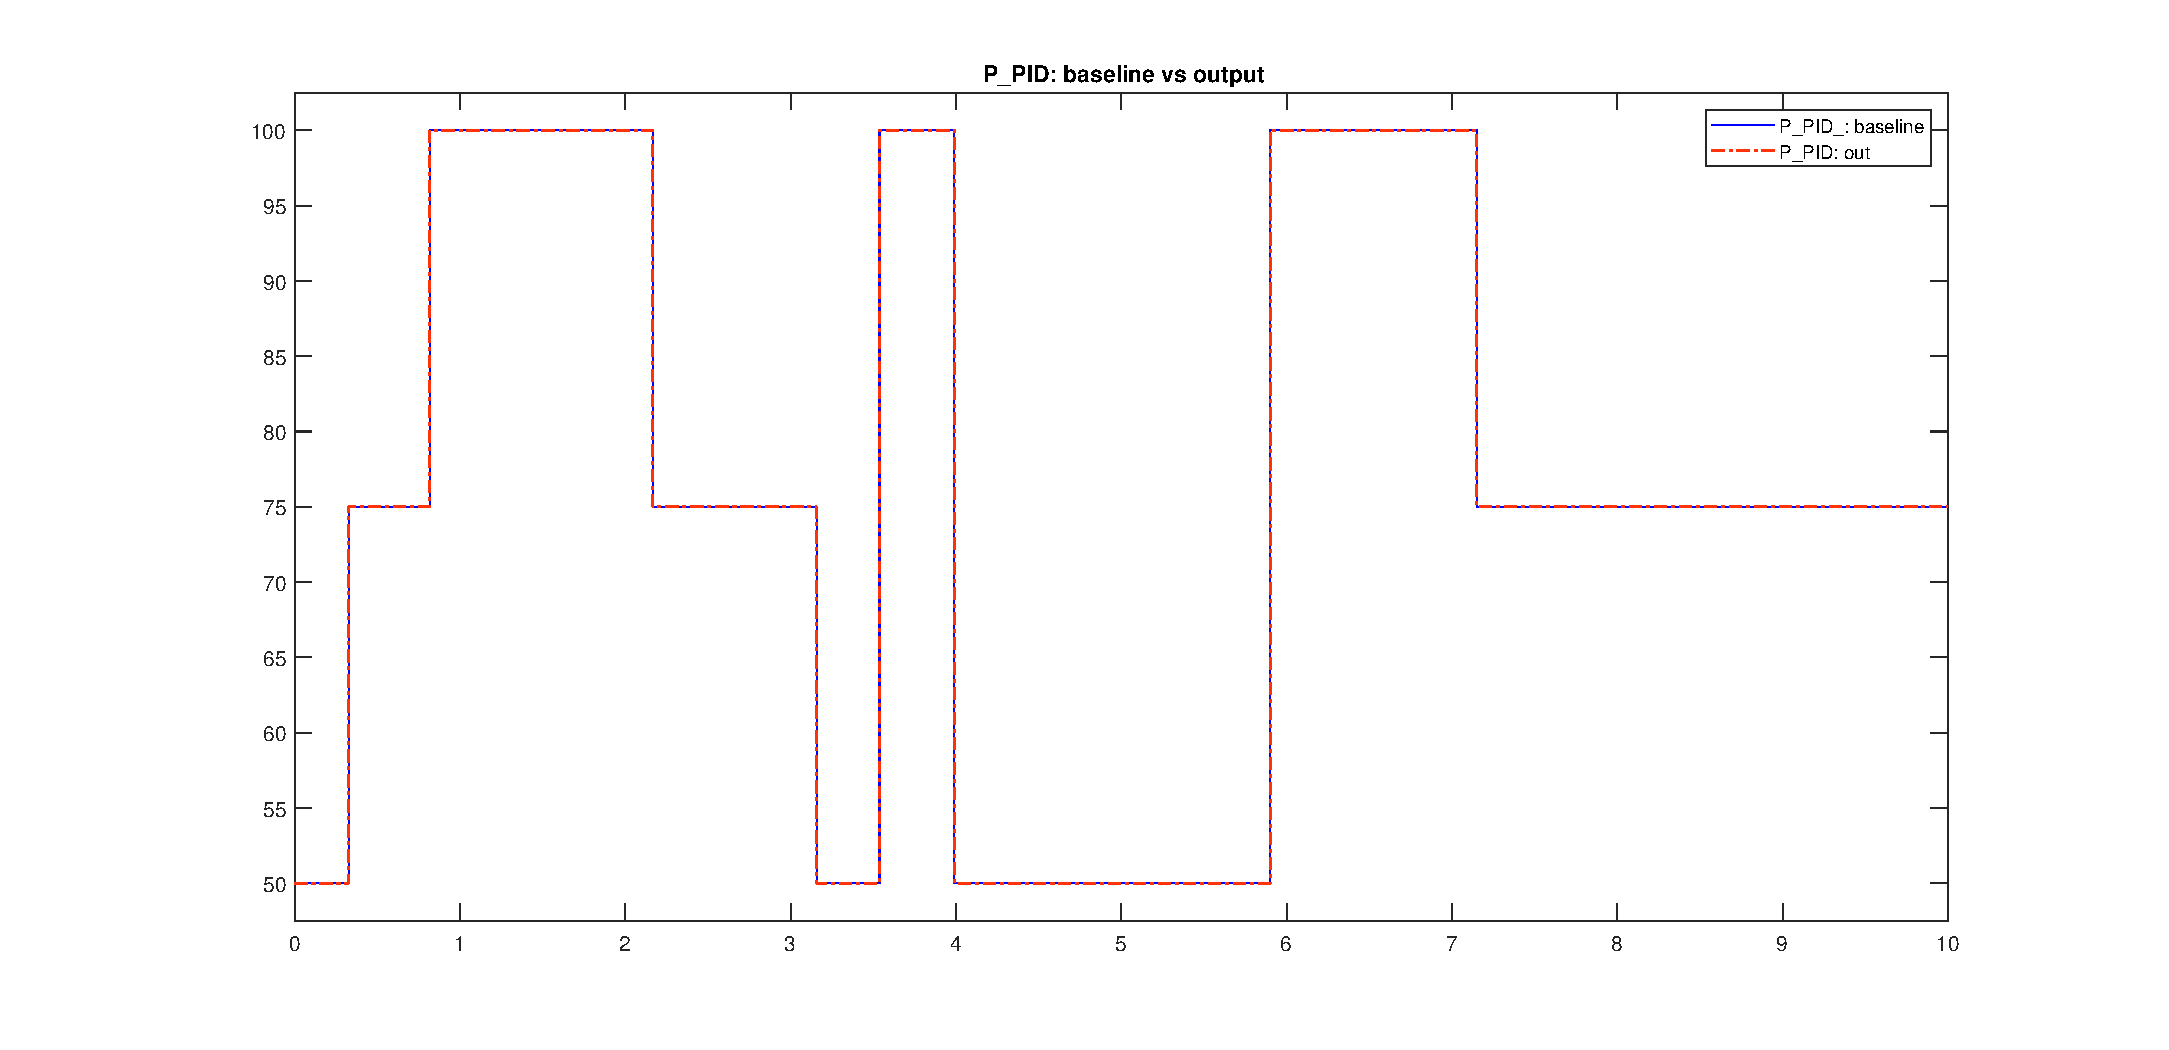
\includegraphics[scale=0.4]{PidP_baseline_result.eps}
	\caption{OTR output vs baseline (up) PID::P output vs baseline (down)}
	\label{OTR_baseline_result}
\end{figure}
We also tested the behaviour of this signal. In Fig.\ref{SoC_handle_input} you can deduce from the input signal (second half of the signal) that we wanted to test that regardless the state in wich we were and the previous value of the SoC signal, the OTR signal would raise when expected to.
In Fig.\ref{OTR_baseline_result} you can see that the output signal matches the baseline, meaning a successful test.
\FloatBarrier
\subsection{Integration test}
All these units cooperate in the same controller module, so an integration test would be necessary. In our specific case these three units do not have in common any input or output, meaning that there is no possible integration test to be performed. All these units are meant to condition the PID behaviour, so in order to perform an integration test the PID would have to be involved. Since we assume the PID block itself already test by MATLAB there is no point in testing the PID behaviour when not regulating a plant model.
According to the previous affirmations we decided to let the integration test coincide with the MIL test, in order to test the behaviour of the whole controller.

\section{MIL}
MIL is a type of testing that can be done at the very fist stage of the development process.\\
It is perform before any software generation code and it does not require any dedicated hardware. For all of these reasons, it is very useful because allow the developers to test their model at the very beginning of the whole process and so, if something fails, time and cost are significantly reduced. \\
In validating the model, the first step that we have to perform is to create the plant of the system (we decided to built it on Simulink). Then, after building the controller, we have to verify that “the controller is able to control the plant” fulfilling all the requirements that were previously discussed. If this happened, the model is verified and we can continue with the next step that will be the SIL.\\
In our case, MIL simulation has the aim to verify the adaptive cruise control. \\
The controller that we implement depends of the speed of the first vehicle and the distance that must be respected between two consecutive vehicles is regulated by the Highway code:\\
\begin{equation*}
	d_s=d_{min}+\dfrac{1}{k}v^2
\end{equation*}
We decided to test the behaviour of the whole system plotting the speed of the first vehicle and the following one. Our high level requirement was that the following vehicle runs accordingly the Highway code, this implies the respect of the safety distance. \\
Since, as mentioned before, the controller take also the SoC value, we decided to plot three different situations depending on the State of Charge of the battery. By doing that, three different responses are shown:\\
\begin{figure}[htbp]
	\centering
	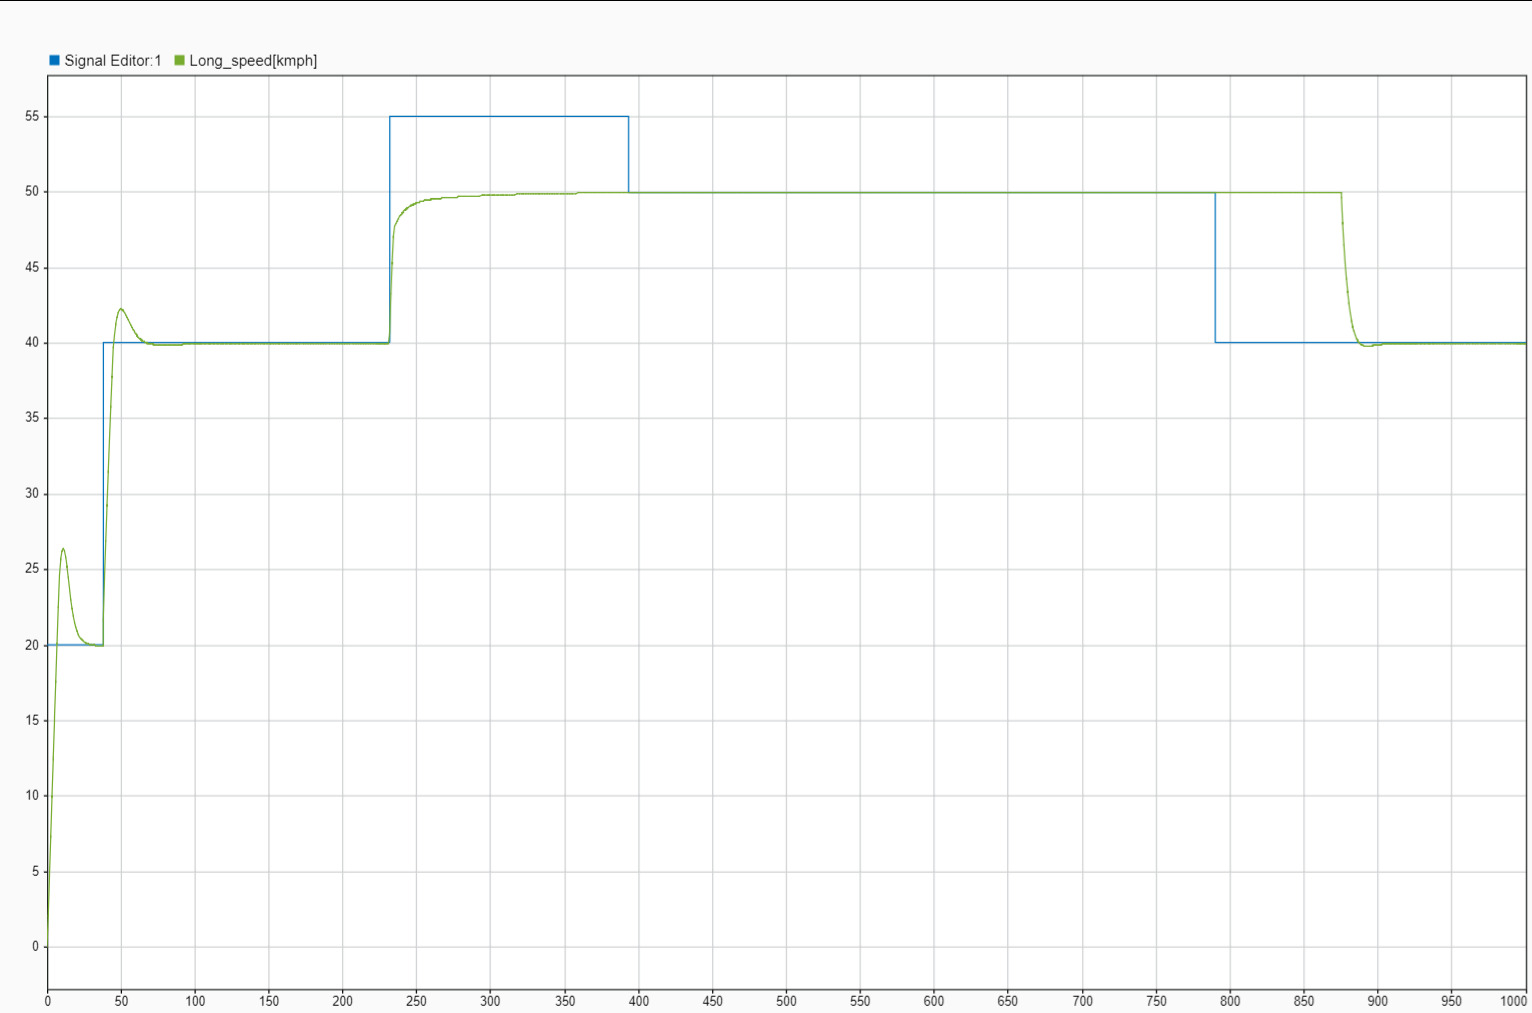
\includegraphics[scale=0.2]{10_soc.jpeg}
	\caption{Speed of the vehicle for 10 SoC}
\end{figure}

\begin{figure}[htbp]
	\centering
	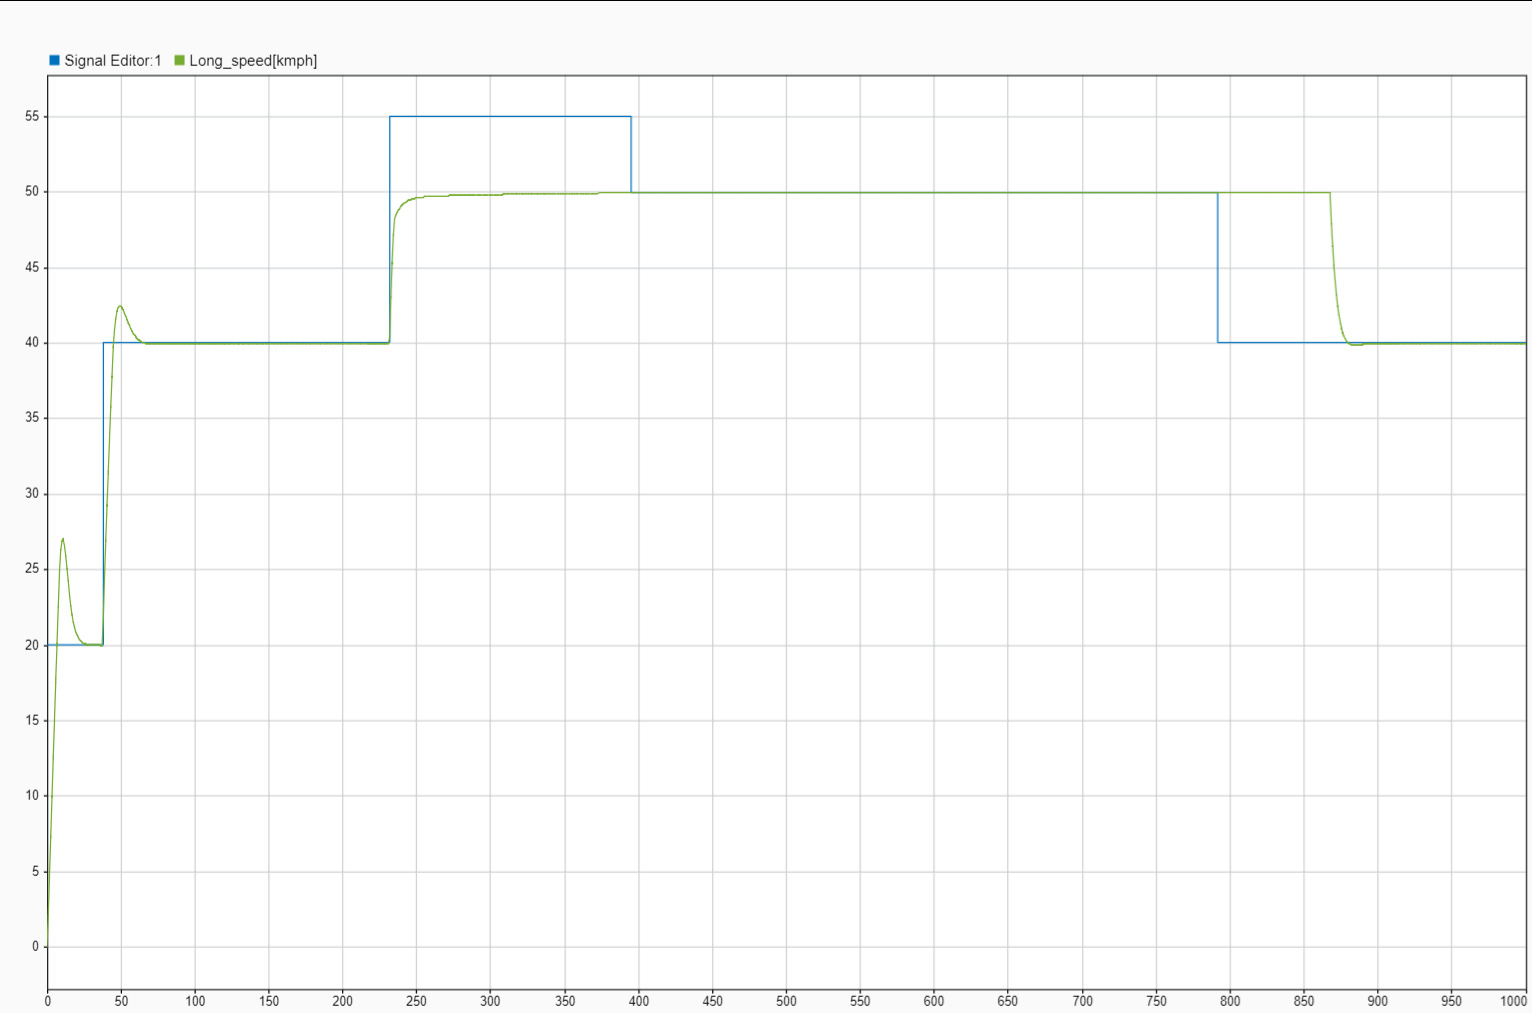
\includegraphics[scale=0.2]{50_soc.jpeg}
	\caption{Speed of the vehicle for 50 SoC}
\end{figure}

\begin{figure}[htbp]
	\centering
	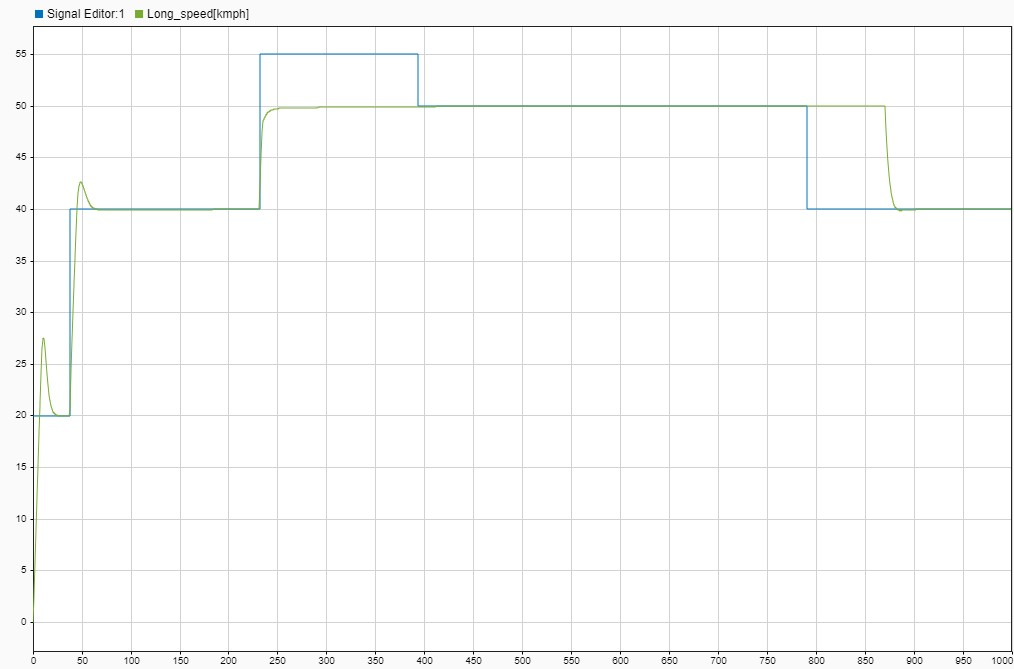
\includegraphics[scale=0.2]{100_soc.jpeg}
	\caption{Speed of the vehicle for 100 SoC}
\end{figure}

As can be seen from the graphs, we implemented our model in order to fulfil all the requirements previously defined: the speed limit imposed by the driver (50 Km/h in this case) is not overcame.\\
In addition, we focused on a particular time interval to show how the SoC value influences the controller response.\\


\begin{figure}[htbp]
	\centering
	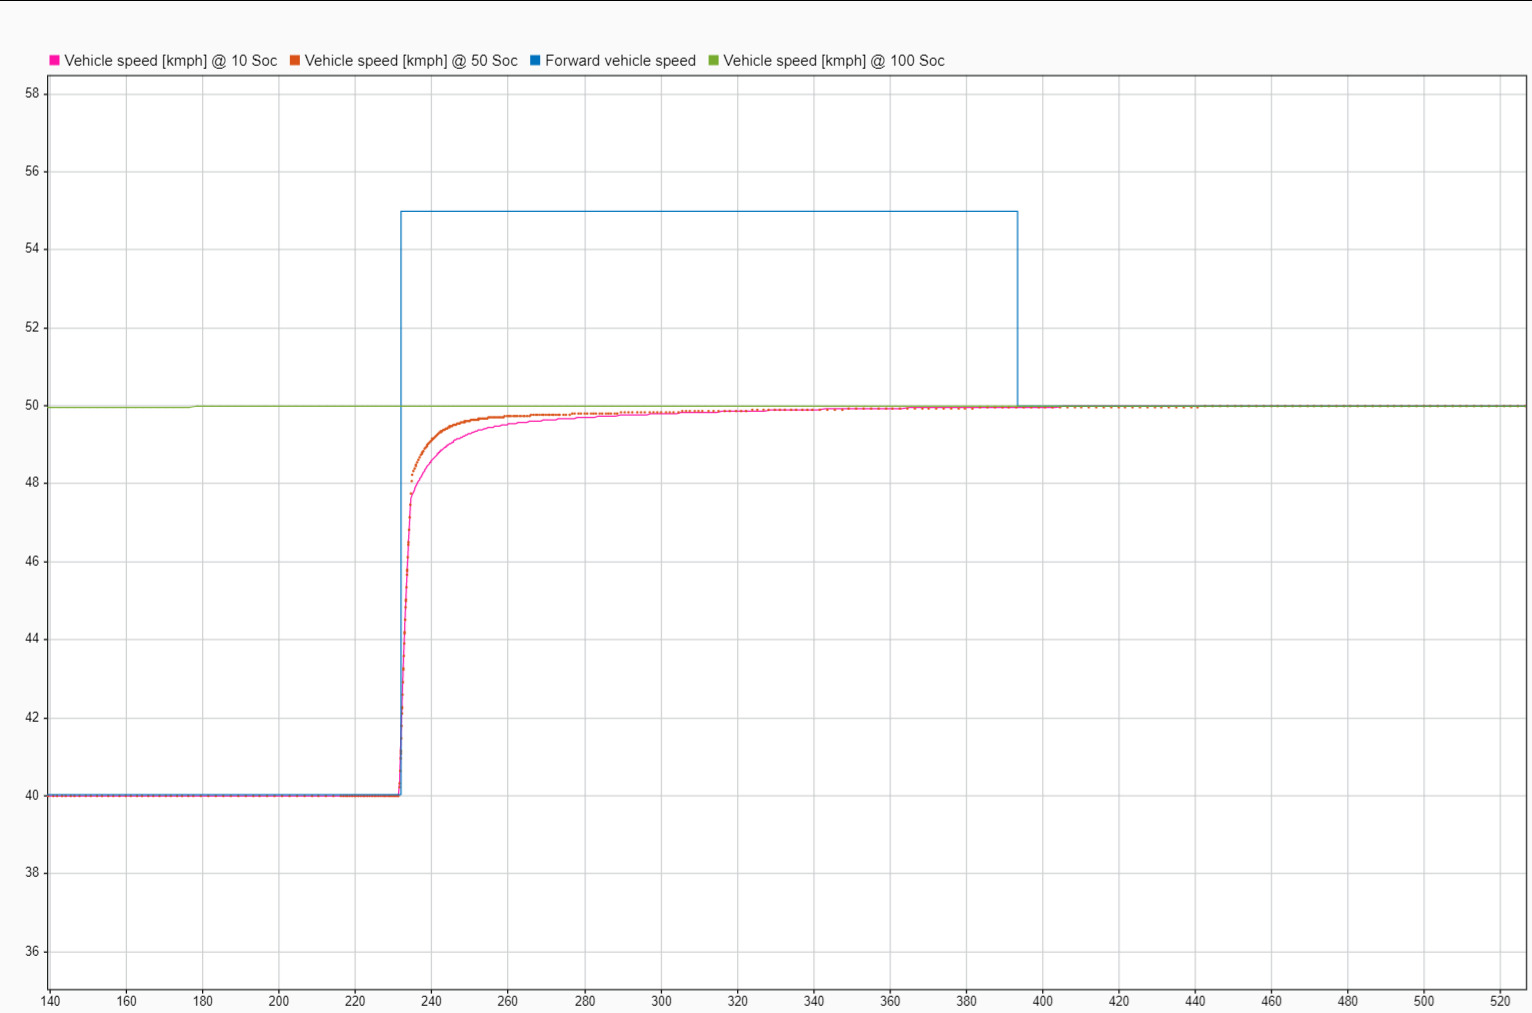
\includegraphics[scale=0.2]{compareSoC.jpeg}
	\caption{Comparison of the speed with different SoC}
\end{figure}

As can be seen from the graphs, where the SoC is higher, the controller can be more aggressive since it can drains more battery. On the other hand, when the SoC is at its minimum, the controller has a smoother and slower response to preserve the battery charge extending its life.


\section{Automatic code generation}
\textbf{Embedded Coder} is on of the tools uses for the automatic generation of code. It is a feature really used by the developers and engineers that automatically generates their code without writing thousands of lines and improve the quality and avoid the errors introduced manually. 
Embedded Coder generate readable, compact and fast C and C++ code for embedded processors. \\
The generated code is ISO C compliant, so it can run on virtually any fixed- or floating-point device and is well suited for applications that need to minimize memory usage or maximize speed. \\
Embedded coder allows to review and navigate from model to generated code and back using code reports with traceability links. It is also possible to verify that the code execution matches model simulation results using software-in-the-loop and processor-in-the-loop testing. SIL and PIL tests can also include code coverage analysis and execution profiling. \\
Embedded Coder offers built-in support for AUTOSAR, MISRA C®, and ASAP2 software standards. In addition, it offers support packages with advance optimization and device drivers for specific hardware.
Matlab and Simulink offer the \textbf{Embedded Coder} to generate C/C++ code from Matlab and Simulink model or subsystem. \\
To generate the code it is possible to estabilish the objectivies using the Code Generation Advisor in order to check that the controller is MISRA C compliant.\\

\subsection{Prepare a Model for Code Generarion}
At first it is needed to prepare a Model for Code Generation:
\begin{enumerate}
	\item Open the \textbf{C Code} tab, click \textbf{Settings} to open the Configuration Parameter dialog blox (or use the shortcut \textbf{Ctrl+E}).\\
	Then select \textbf{Simulation $\to$ Model Configuration parameters}
	\item Open the \textbf{Solver} pane and select:
	\begin{itemize}
		\item \textbf{Solver type}: Fixed-Step.
		\item  \textbf{Solver}: discrete.
	\end{itemize}
	\item Open the \textbf{Optimization} pane, and set Default parameter behavior to Inlined.
	\item Open the \textbf{Code Generation} pane, and specify ert.tlc as the System Target File.
	\item Clear \textbf{Generate makefile}.
	\item Select \textbf{Generate code only}.
	\item Enable the HTML report generation by opening the \textbf{Code Generation $\to$ Report} pane and selecting Create code generation report and Open report automatically. Click the horizontal ellipsis and, under Advanced parameters, select \textbf{Code-to-model}. Enabling the HTML report generation is optional.
	\item Click Apply and then OK to exit.
\end{enumerate}
\subsection{Generate Code using Ebedded Coder}
The steps that must be followed are:
\begin{enumerate}
	\item Open the model that contains the block. 
	\item In the Code Generation Advisor, click Set Objectivies. Is an important step in which it is possible to check the coding standard compliance. There are different objectivies that can be selected and it is possible to select and prioritize the combination of objectivie before generating the code.
	\item On the C Code tab, click Quick Start.
	\item In the Generate Code step, apply the proposed changes and generate code by clicking Next.
	\item Click Finish, then return to the C Code tab. From this it is possible to configure code generation customizations, and then check the results in the Code view next to the model.
	\item With the right clock o the component it is possible to build the process and going to C/C++ Code Generation, then click on \textbf{Build}.
	\item View the code generation report.
\end{enumerate}
\section{Software-in-the-loop Simulation (SIL)}
A software-in-the-loop (SIL) simulation compiles generated source code and executes the code as a separate process on a target host computer. By comparing normal and SIL simulation results, it is possible to test the numerical equivalence of the model and the generated code.
Thanks to the \textbf{Embedded Coder Toolbox} there are different ways to perform a SIL simualtion. \\
Throught a communication channel, Simulink sends stimulus signals to the code on the computer or target process for each sample interval of the simulation:

\begin{itemize}
	\item Top-model (SIL simulation generates the stanalone code interface) and Model block. For both, the Test behavior of generated source code on development computer. Execution is host/host and nonreal time.
	
	\item SIL or PIL block (block uses standalone code interface). In this case the Simulation runs compiled object code through S-function. S-function communicates with object code executing as standalone application on development computer. Execution is host/host and nonreal time.
\end{itemize}


The method used in this report is the creation of a SIL block. \\
In the model setting it is needs to use the Embedded Coder in the Code Generation section (ert.tlc).\\
\begin{figure}[htbp]
	\centering
	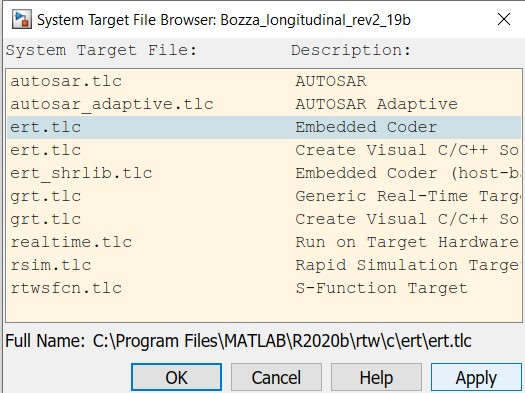
\includegraphics[scale=0.7]{ert.jpg}
	\caption{Target selection}
\end{figure} \FloatBarrier

Then it is possible to check the hardware implementation and check the host architeture on which automatically generated code for the controller will running. \\
The follow step is to check a specific flag in the Code Generation section, in particular in the Verification in which it is possible to select the creating block. 
After that, clicking on the unit, in the C/C++ Code, clicking $Build$ creates the SIL version of the Controller subsystem block. \\
After the creation of the SIL block, a comparison simulation has been carried out. The entire plant has been simulated and then it is possible to observe the error between the two different simulations. \\

The following steps summarize the creation of a SIL block:
\begin{enumerate}
	\item From the Configuration Parameters $\to$  Code Generation $\to$  Verification $\to$  Advanced Paramters $\to$  Create block drop-down list, select the SIL block.
	\begin{figure}[htbp]
		\centering
		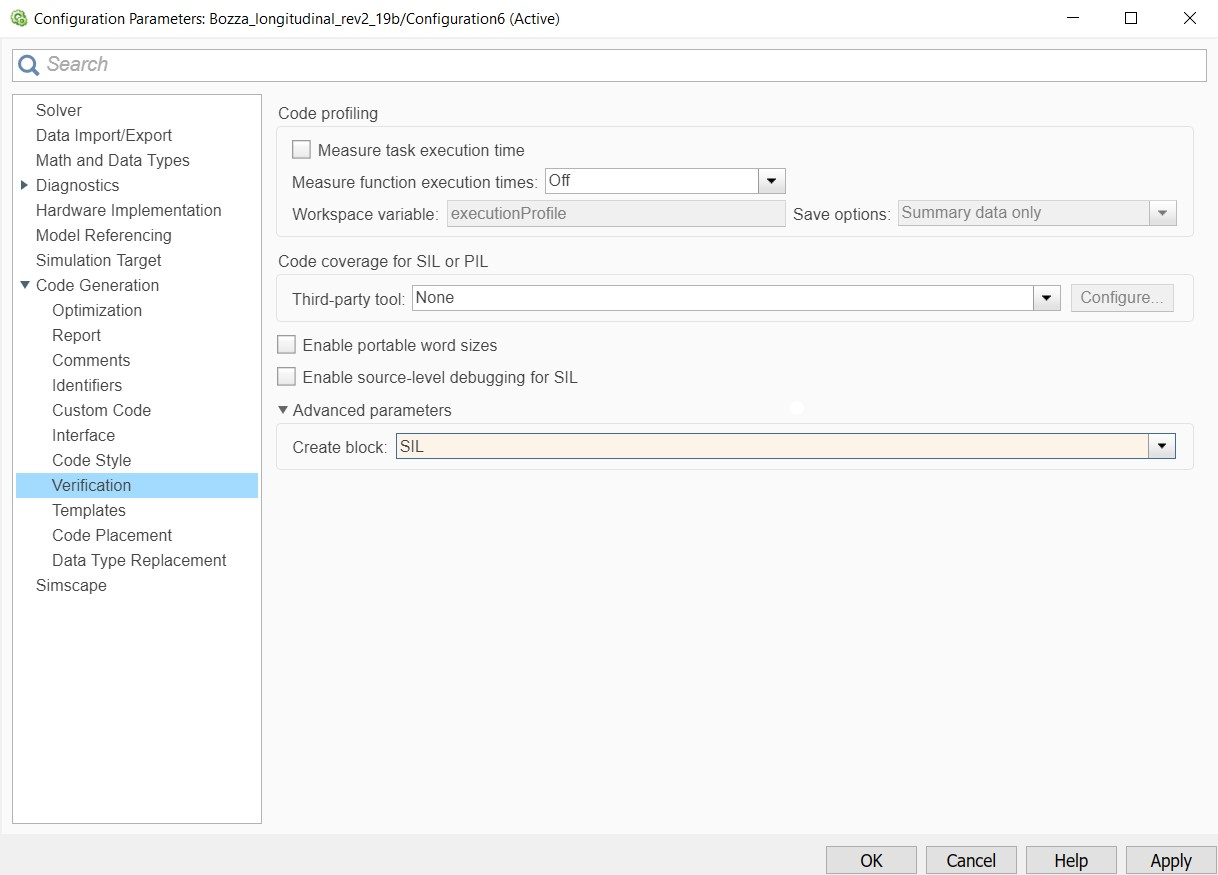
\includegraphics[scale=0.4]{verification.jpg}
		\caption{Creation of the SIL block}
	\end{figure} \FloatBarrier
	\item Click OK.
	\item In the model window, right-click the subsystem that it is need to simulate.
	\item Select C/C++ Code $\to$  Build This Subsystem.
	\item Click Build, which starts the subsystem build process that creates the SIL block for the generated subsystem code.
	\item Add the generated block to the environment.
	\item Run the simulation with the environment.
\end{enumerate}

The simulation results are represented in the following figure:
\begin{figure}[htbp]
	\centering
	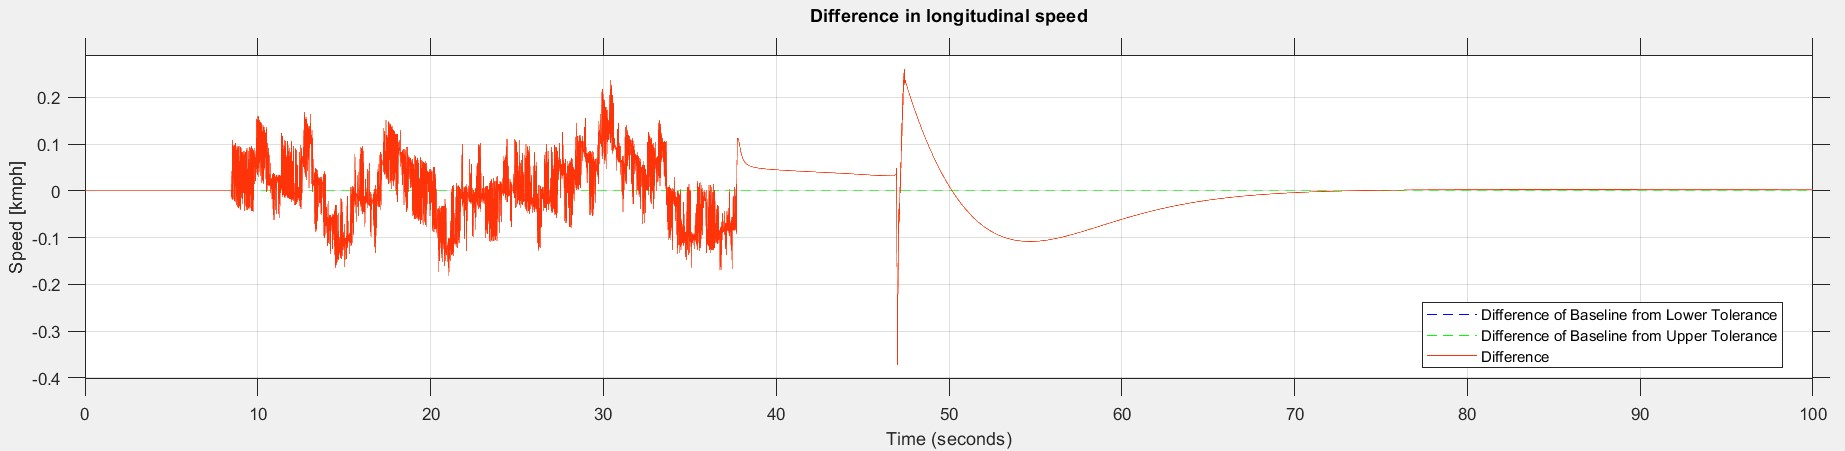
\includegraphics[scale=0.4]{sil_plot.jpg}
	\caption{Difference in longitudinal speed of the original Simulink model and the SIL model}
\end{figure} \FloatBarrier

It is possible to see that the difference between the two simulations is negligible, so the whole result is acceptable.
\section{Processor in-the-loop Simulation (PIL)}

The chosen hardware for the simulation is the Raspberry Pi 4 model B, equipped with quad-core processor (ARM-cortex), is wireless connected to PC.
To provide a stable connection between hardware and Simulink it is necessary to set properly the device address (IP address) and the credential of the OS system for privileged read/write operation.


\begin{figure}[htbp]
	\centering
	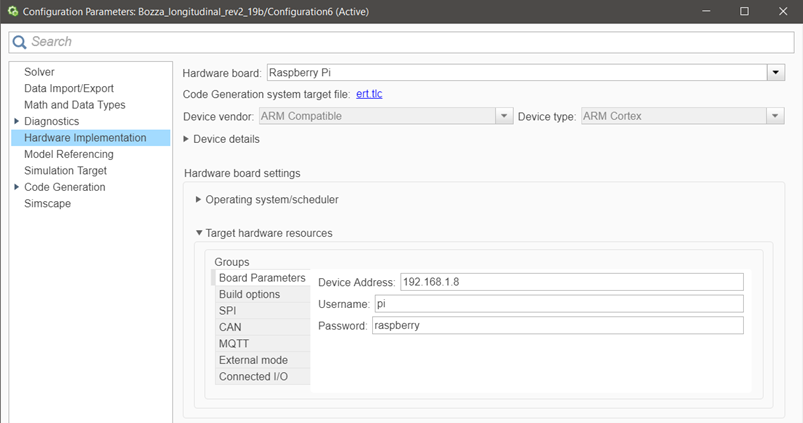
\includegraphics[scale=0.8]{hw_implementation.png}
	\caption{Hardware settings}
\end{figure} \FloatBarrier

The generation of the code is widely described above on the SIL section and the procedure for generation of the PIL block is the same as for SIL.

\begin{figure}[htbp]
	\centering
	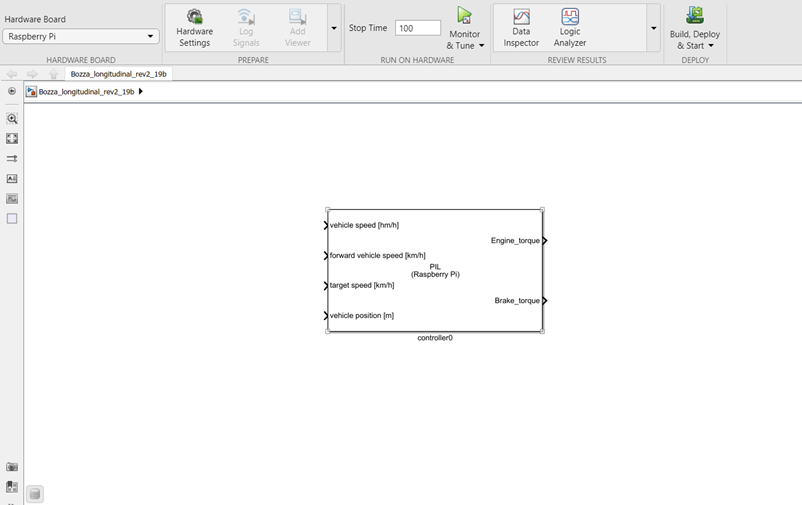
\includegraphics[scale=0.7]{PIL_block.png}
	\caption{PIL block}
\end{figure} \FloatBarrier
Once the controller is replaced by PIL block, the entire code is deployed on Raspberry board and the simulation starts. 
\begin{figure}[htbp]
	\centering
	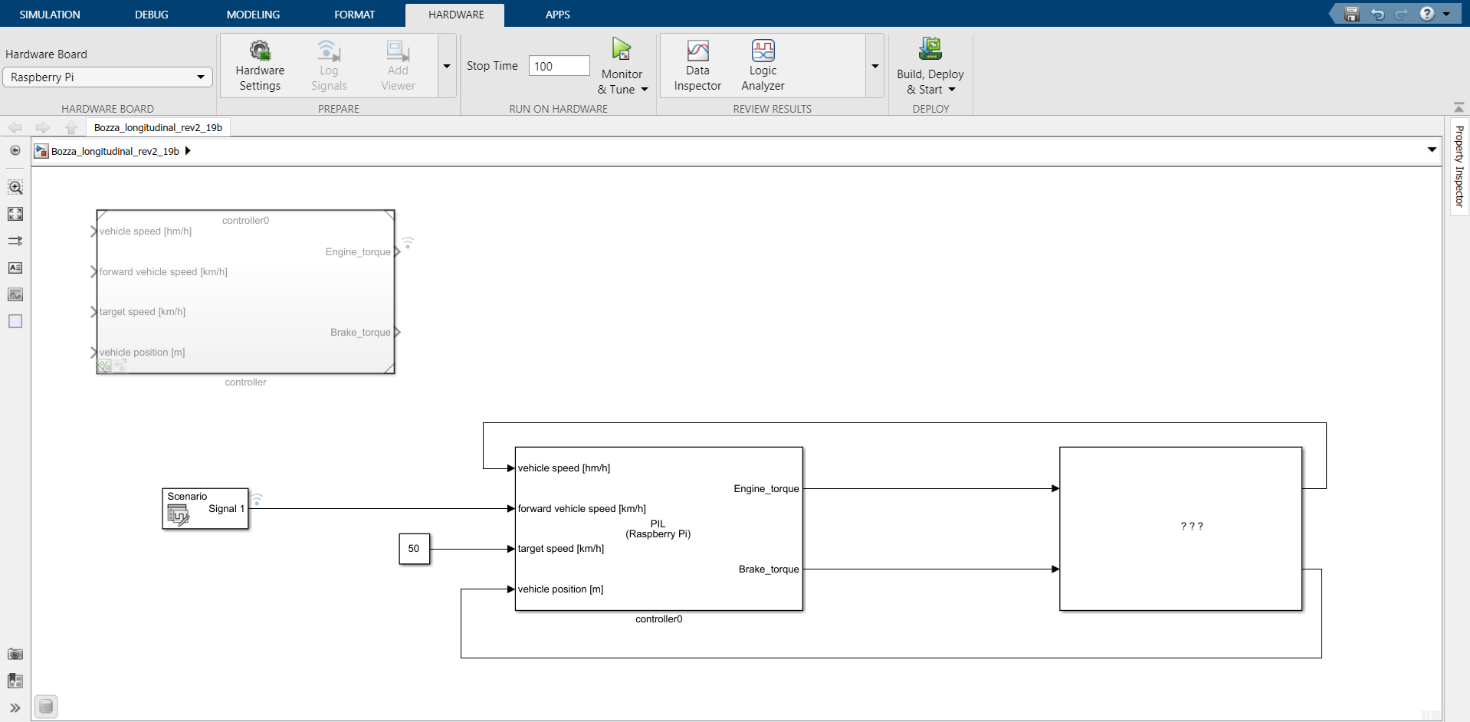
\includegraphics[scale=0.7]{PIL_sim.png}
	\caption{Simulation PIL block}
\end{figure} \FloatBarrier
From the comparison simulation can be noticed the difference between the longitudinal speed of original Simulink model and the one of PIL model.
\begin{figure}[htbp]
	\centering
	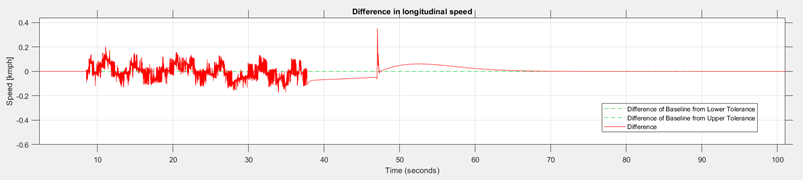
\includegraphics[scale=1]{plot_PIL.png}
	\caption{Difference in longitudinal speed of the original Simulink model and the PIL model}
\end{figure} \FloatBarrier

The overall result is acceptable.
The difference between the two simulation is negligible and bounded in a very short range.

\chapter{Conclusion}
	
	
\end{document}
